\chapter{Learning to reason with uncertainty as humans}
%
%	Need to make this stick with the previous Chapter !
%
%	-> 
%
The conclusions drawn from the literature survey in Chapter 2 are that non-heuristic methods for planning and control 
rely heavily on the initial data provided to their respective optimisers. An ideal initial set of behaviour should be comprised
of explorative and exploitative actions so that a final optimal policy can quickly achieve the balance between minimising 
uncertainty and solving the task at hand. This is especially true for Reinforcement Learning (RL) methods which make use of 
explorative actions to be able to find an optimal policy. In many RL applications random exploration or Gaussian noise perturbation
is sufficient to find an optimal policy. This is the case when either an exhaustive search of the action space is possible 
(mountain cart, inverted pendulum, etc...) or in policy search methods where the policy is parametrised by a few parameters.
In continuous action-state space POMDPs, when a generic non-parametric policy is desired  this is not practical, especially 
when the decision horizon is long. Continuous action-state space POMDPs applications have predominantly focused on cases in which 
the uncertainty can be quantized by a single Gaussian parametrisation. This representation can be constraining since it requires 
the observation likelihood to be Gaussian as well. This assumption is restrictive and ill-suited for haptic search tasks in 
which observations are discontinuous and occur as impulses. 

In this chapter, we demonstrate that human foresight and intuition can be leveraged as a means of solving the 
exploration/exploitation dilemma under partial observable conditions. Human beings are versatile in their ability to 
accomplish tasks which are considered to be complex by current robotic standards. This perceived ability which we have over 
current robotic systems, due to our prior domain knoweldge and experience, can be extracted, encapsulated and transferred 
to a robot apprentice. This chapther has been published in \cite{deChambrierBillard2013,Chambrier2014}.

To demonstrate the application of the transfer of behaviour from a human teacher to a robotic apprentice we apply the framework outlined in Chapter 2, 
Section \ref{sec:approach} (PbD-POMDP) to a blindfolded haptic search task. In our blindfolded search task, both a robot and a human 
must search for an object on a table whilst deprived of vision and hearing, illustrated in Figure \ref{fig:searching}. 
The robot and human both have prior knowledge of the environmental setup making this a specific search problem with no required mapping of the environment, also known as active localisation. 
In Figure \ref{fig:searching}, a human has his sense of vision and hearing impeded, making the perception of the environment partially observable and 
leaving only the sense of touch available for solving the task. The hearing sense is also impeded since it can 
facilitate localisation when no visual information is available and the robot has no equivalent giving an unfair 
advantage to the human. By impeding hearing we align the perception correspondence between the human and robot.

By representing the belief of the human's position in the environment by a Particle Filter (PF) and learning a mapping from this belief 
to hand actions (velocities) with a Gaussian Mixture Model (GMM), we can model the human's search process and reproduce it for any agent. 
We further categorize the type of behaviours demonstrated by humans as being either risk-prone or risk-averse and find that more than 70\% of 
the human searches were considered to be risk-averse. We contrast the performance of this human-inspired search model with respect to Greedy and Coastal Navigation search methods. 
Our evaluation metric is the distance taken to reach the goal and how each method minimises the uncertainty.
We further analyse the control policy of the Coastal Navigation and GMM search models and argue that taking  uncertainty
into account is more efficient with respect to distance travelled to reach the goal.

\begin{figure}[h]
  \centering
  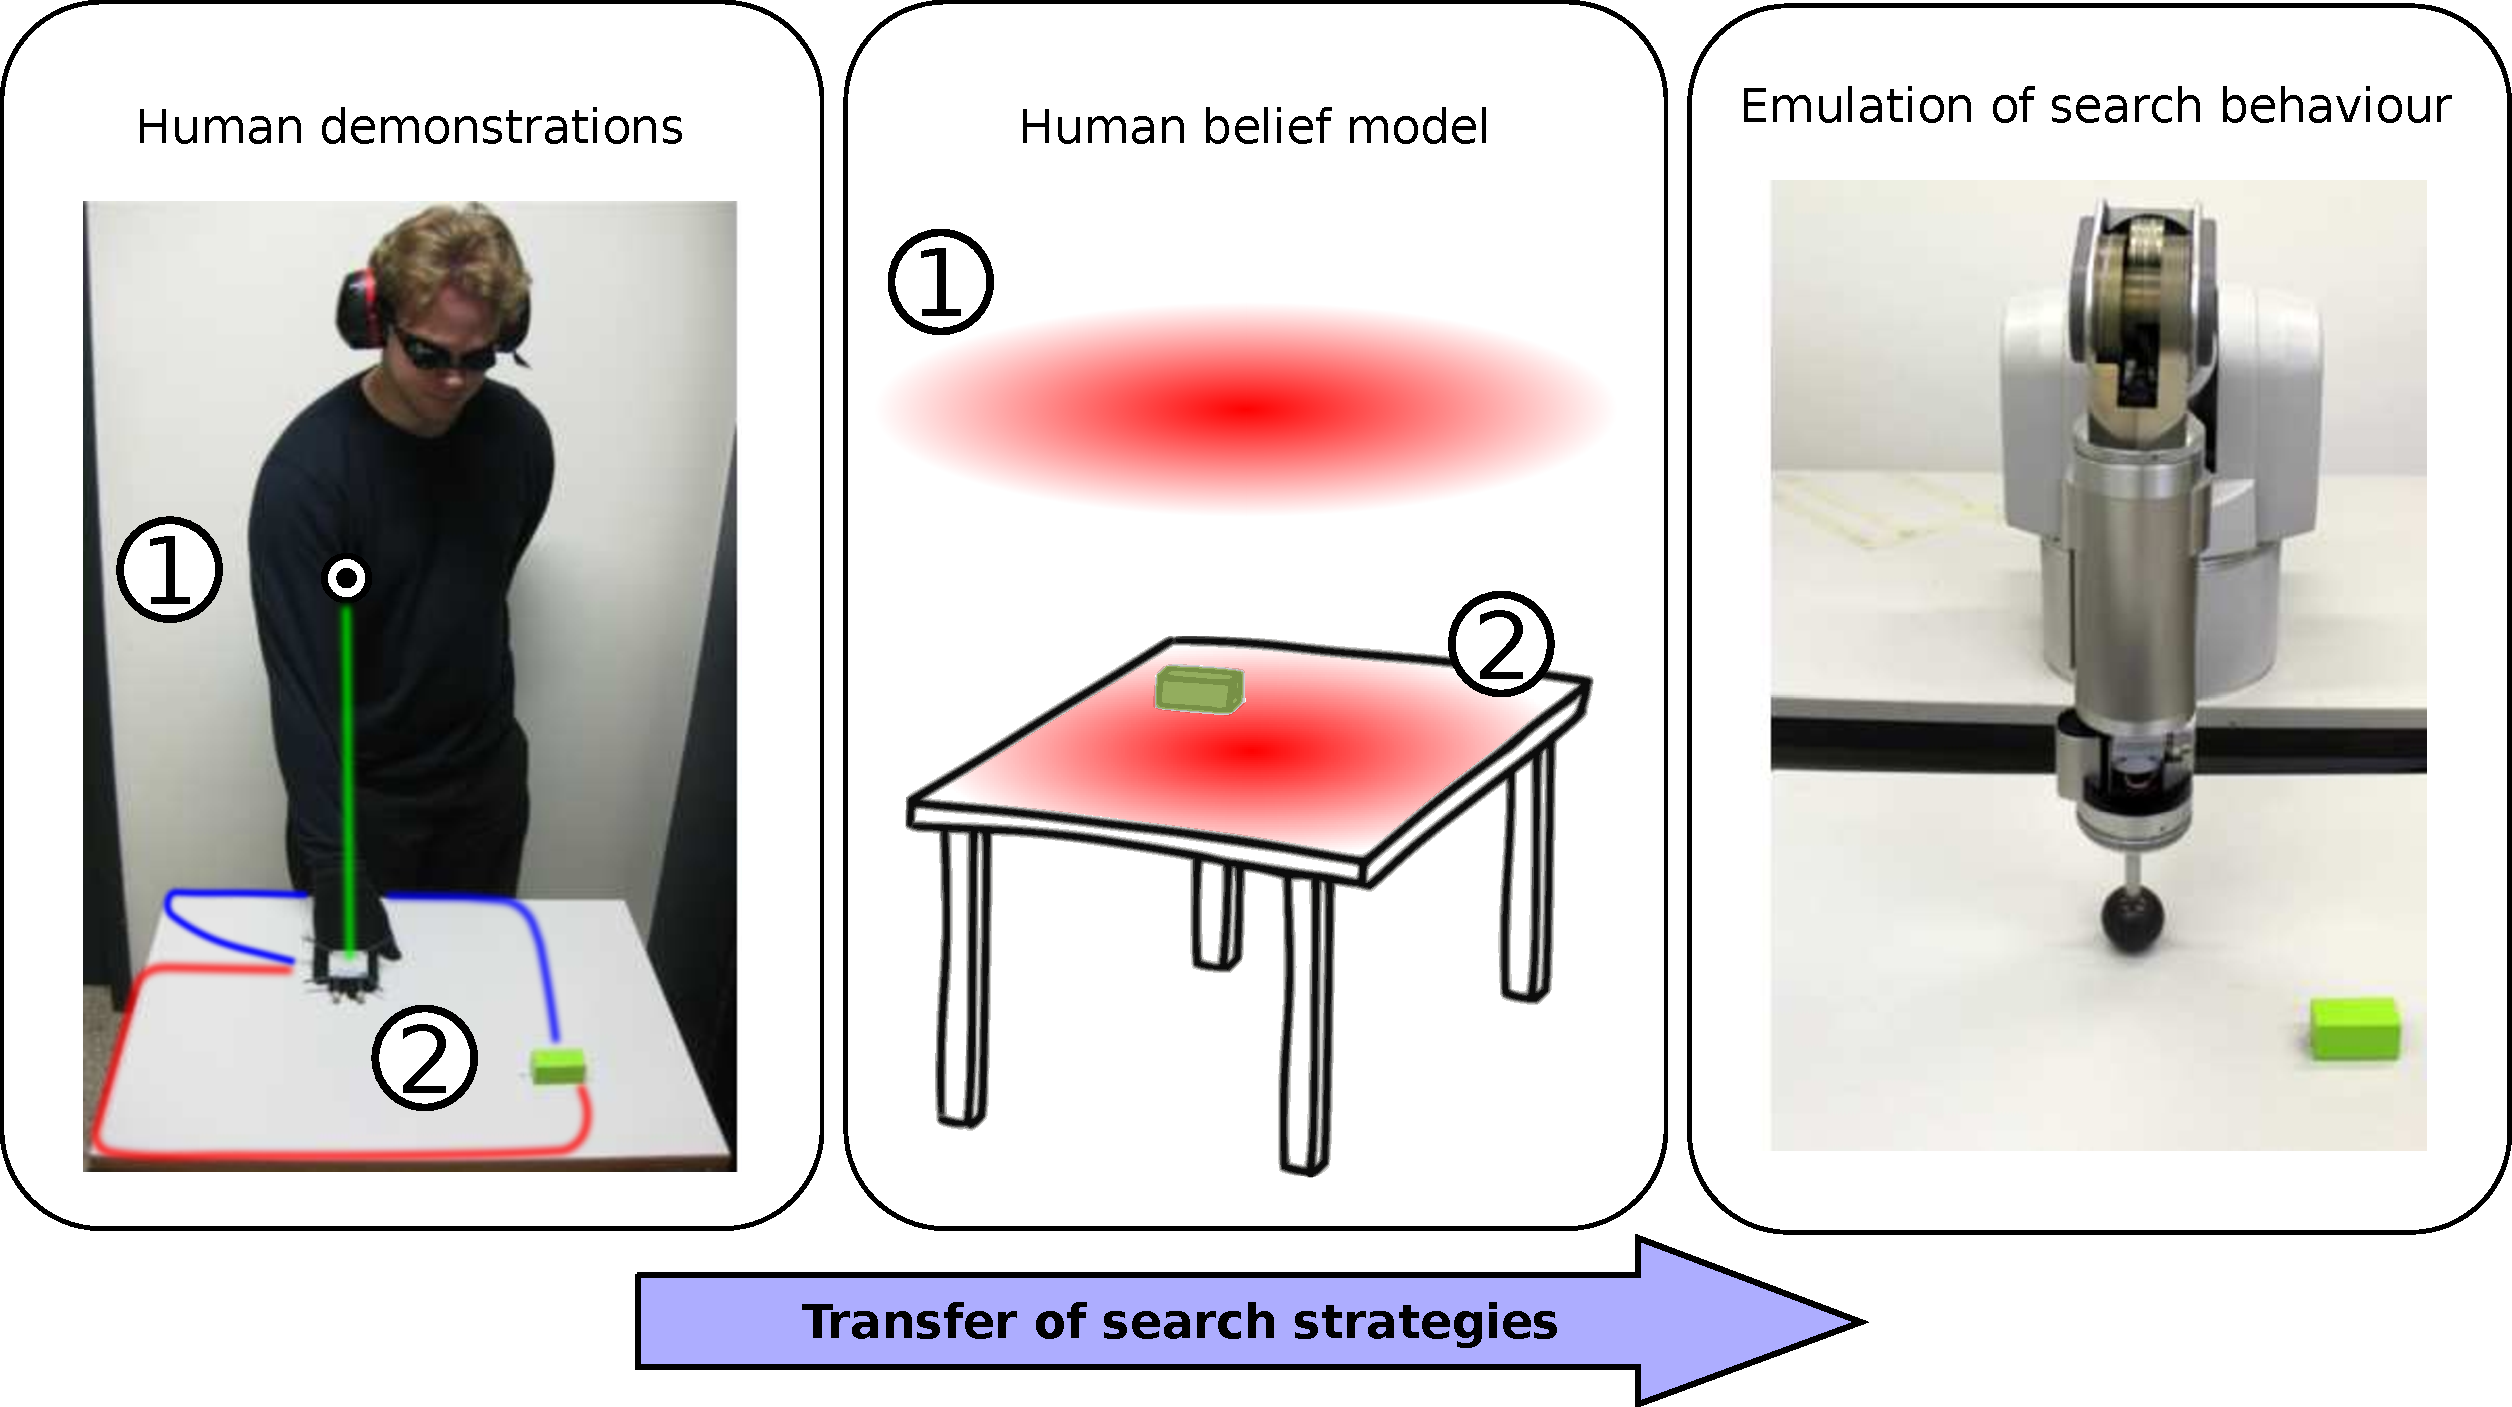
\includegraphics[width=0.95\textwidth]{./ch3-Search/Figures/Figure1.pdf}
  \caption{\textbf{Blindfolded search task} \textit{Left:}  Search task, a human demonstrator searching for the green wooden block on the table given
  that both his hearing and vision senses have been impeded. He starts (hand) at the white spot near position (1). The the red and blue trajectories 
  are examples of possible searches.
  \textit{Middle:} Inferred belief the human might have with respect to his position. If the human always starts at (1) and his belief is known, all 
  following beliefs (2) can be inferred from Bayes rule. \textit{Right:} WAM Robot 7 DOF
  reproduces the search strategies demonstrated by humans to find the object.}
 \label{fig:searching}
\end{figure} 

There are \textbf{two assumptions} we make when applying Programming by Demonstration, PbD (also known as Imitation Learning), to the POMDP task described above. 
The first assumption is that the human teacher's \textit{spatial cognitive} abilities are good enough to accomplish 
the task in a consistent fashion. In other words demonstrations should not be random and a pattern exists. The second assumption is that human beliefs inferred  
by the apprentice are close to the actual belief of the human. 

\section{Outline}

\begin{itemize}

\item  \hyperref[ch3:background]{\ref{ch3:background}   Background}\\
We review aspects of the literature in robotics and cognitive science which are related to spatial navigation which 
consider scenarios with limited perceptual information. We review related literature from \textit{Spatial Navigation}, 
\textit{Theory of Mind} and \textit{Programming by Demonstration}.

\item  \hyperref[ch3:experiment]{\ref{ch3:experiment}   Experiment}\\
The table search experiment protocols are described and we detail how to learn and transfer search strategies from human teachers to a robot 
apprentice. A total of 15 human teachers participated and each gave 10 demonstrations, giving a total of 150 searches.

\item  \hyperref[ch3:formulation]{\ref{ch3:formulation}  Formulation}\\
We detail the implementation of the human belief in terms of a Particle Filter (PF). This includes the measurement and motion 
models. We describe how we compress the belief particle filter in terms of the most likely state and differential entropy.

\item  \hyperref[chap3:policies]{\ref{chap3:policies} 	Policies}
\begin{itemize}
  \item \hyperref[chap3:GMM_policy]{\ref{chap3:GMM_policy} Modelling human search strategies}\\
  We detail the implementation and parametrisation of a Gaussian Mixture Model (GMM) policy encapsulating
the human search strategies and how it synthesises new searches.
  \item \hyperref[chap3:costal_policy]{\ref{chap3:costal_policy} Coastal Navigation}\\
  We detail the implementation of a Coastal Navigation policy, used as a comparison with the GMM policy.
\end{itemize}

\item  \hyperref[chap3:results]{\ref{chap3:results} 	Results}\\
We conduct three types of analysis: we quantify the behaviour present in humans and policies in terms of riskiness; we 
qualitatively evaluate the differences between the GMM policy learned from human demonstrations and the Coastal Navigation policy;
we evaluate the distance taken to find the goal for a set of four search policies, including the GMM.

\end{itemize}
\clearpage
\section{Background}\label{ch3:background}

%\subsection{Acting under partial observability}
%Learning controllers or policies to act within a context where the state space is partially observable is of high relevance to all real 
%robotic applications. Resulting from limited and inaccurate perceptual information, often only an 
%approximation of the environment is available at any given time. If this inherent uncertainty is not taken 
%into account during planning or control there is a non-negligible risk of missing goals, getting lost and 
%wasting valuable resources. 



%A major difficulty faced in spatial cognitive navigation and within the context of our PbD-POMDP framework is that 
%the biological and neurological processes which are responsible for the observed behaviour during the experimental studies 
%are unobservable. Even with the increasing usage of neuro-imaging techniques such as functional Magnetic Reasons Imaging (fMRI)
%and electroencephalogram (EEG), whose technical aspects impose limitations on the possible experimental studies, it is hard to 
%determine a cognitive mathematical model of the underlying processes present in spatial navigation. 

\subsection{Spatial navigation}
%
%	Take away points: 1) Humans and animals are currently better than robots in doing this.
%		          2) Limitations of the quality of our policy depend on our working memory.
%

Spatial navigation, \cite{Wang_2007}, \cite{what_det_our_nav_ability_2010}, focuses on the role that sensory perception 
(vision, vestibular, proprioception ...), motor control and mental cognition have on the navigational ability of  
humans, animals and insects. A central aspect of spatial navigation is the way in which we mentally represent the geographical world, known 
as a \textit{cognitive map} (mental representation of environment first proposed by Tolman, 1948) and how we update our pose estimation 
in this map. The aspects of both  construction and correction of a cognitive map have been studied in great depth, \cite{spatial_updating_2008}.
There is reported evidence that we use both vestibular and proprioception in inferring self-motion in order to update our position through dead reckoning (also known as path integration). 
Given the estimated position we then use external cues such as geometric (the shape of a room) and features (the colour of the walls), 
to correct our position. The actual representation of our position and environment in our cognitive map has been proposed,
\cite{spatial_memory_how_ego_allo_combine_2006}, to be either encoded in our own frame of reference (egocentric) or in a frame of reference which 
is independent to us (allocentric) and acts like a standard paper map or both. This cognitive map enables us to reason about the relations between our own position and that of other items and landmarks present. 
This representation also facilitates our ability to localise ourselves and plan novel routes when needed.

In \cite{updating_egocentric_human_navigation_2000}, the authors studied the effect that disorientation has on blindfolded subjects' ability 
to recover their heading, which is necessary for re-localisation. Through eight different experiments they concluded that humans 
have an egocentric cognitive map.


Studies have also looked at the difference between congenitally blind, late blind and sighted people in their ability to encode ego-allocentric cognitive maps.
In \cite{Pasqualotto2013175}, the authors dispose a set of seven objects (brush, slipper, pan, dish, book, spoon, bottle) in the form of 
an array in a 12.5m $\times$ 9m room. The objects are positioned on top of stools. During a training phase, ten congenitally blind, ten late blind and ten blindfolded sighted people were taken through 
the setup and touched all objects present. This guided exploration (the experimenter leading the subject through the object array) was repeated until 
the participants could correctly recall all the objects' locations twice consecutively without help. In a testing room (no objects present) 
the participants were asked ``Judgement of Relative Direction''  questions and the accuracy and response time were recorded. From the results the authors 
concluded that blindfolded and late blinded participants used a allocentric representation of the object array, whilst the congenital blind 
subjects use an egocentric model. The cause of this difference is attributed to the role played by vision in the development of the 
multisensory brain area, in which vision is necessary for the development of an allocentric model. 

Many similar experiments have been conducted and a summary can be found in the following review \cite{spatial_memory_how_ego_allo_combine_2006},
where the authors explicitly state that a consensus has formed; both egocentric and allocentric representations of the environment are 
working in parallel. Current questions ponder whether allocentric models are part of the semantic memory as opposed to the procedural 
memory used by the egocentric model.

\subsubsection{Spatial cognition and memory}

The quality of the human teacher in  search tasks, which are partially observable in the terms of absence of vision,
will strongly depend on the teacher's ability to maintain an accurate cognitive map of his environment. This implies
that the size of the environment and search task will have an effect on the teacher's ability to provide near optimal 
demonstrations. 
Early and influential research into human's short term memory was presented in 1956 by George Miller in a seminal work, \cite{cogprints730} 
(22'780 citations), in which he described the ``so called'' magical number of our short term memory as being $7\pm2$ items, 
known as \textit{Miller's Law}. This research was conducted on a  one dimensional task in which no spatial navigation was required.
Since then there have been many studies investigating the limits of short term memory.

In \cite{human_stsm_2015} a set of subjects had to find either 1, 3, 5 or 7 goal pads, among a grid array of 23 pads in a 4m $\times$ 4m room, 
within a one minute interval. They measured the subjects' error in terms of the number of locations visited before finding the goals. 
They found that on average the subjects had to visit ``$1.6 \times \#num\_goals$'' pads before achieving the task. The authors concluded 
that in this spatial navigation task there was no magical number which represents the limit of short term memory.
In another spatial navigation experiment, \cite{Iachini2014}, the effect that the scale of the environment 
has on the ego-allocentric representation is studied in blindfolded, late and early blind subjects. The main findings were
that cognitively blind people have more difficulty in developing an allocentric representation of the world. 
%In terms of difference in the scale of the problem (two conditions where compared, a task which required no locomotion and one that did), 
%only a small difference existed for the blindfolded subjects.

In \cite{stankiewicz2006lost}, a search task in a virtual maze is conducted by a set of human subjects.  The aim 
is to investigate the limitations that perception, memory and uncertainty have on human decisions in comparison 
to an ideal agent (POMDP solution). The authors' main findings were that as the size of the maze increases the
performance of the human subject decreases with respect to the ideal agent, as human subjects are limited by the 
uncertainty in their location and have difficulty in maintaining multiple hypotheses.

\subsubsection{Summary: spatial cognition}


The studies detailed above reported that if the environment is not overly large and complex our cognitive model is sufficient 
to produce policies which are on par with an optimal POMDP agent. 

Our study seeks to transfer exploratory behaviour from human teachers to a robot apprentice in a partially observable setting. 
In our search scenario the environment is less than 3 meters in length and 2 meters in depth with a single goal object to be found. 
Given this setup and the evidence from previous studies, humans should be able to achieve this task with a high level of proficiency. 

This is beneficial since currently both humans and animals are better at spatial navigation than robots \cite{stankiewicz2006lost} 
especially when uncertainty is present. The quality of the demonstrations will strongly depend on the teacher's short term memory 
in retaining a sufficiently accurate cognitive map of the environment. 


\subsection{Human beliefs}

% Belief  
%In the Section \ref{sec:deci_un} on Decisions in Chapter 2, we introduced the concept of rationality for 
%both beliefs and desires. 

A crucial aspect for the success of PbD-POMDP learning is that the apprentice be able to infer 
the human's belief of his location whilst he is searching. In others words the apprentice
(human or robotic) has to infer the cognitive map of the teacher. 

%This is possible by observing the actions of teacher and guessing his perception 

The study of inference of another's mental state is part of Theory of Mind (ToM) \cite{Towards_a_ToM_2010}, which is concerned 
with our ability to infer beliefs, desires, intentions, perception,
goals and current knowledge. In this study, the apprentice will have to infer the teacher's beliefs which we assume are 
\textbf{rational}. A rational belief is a belief for which observations bring supportive evidence and 
gradually increase the certainty of the belief. In a recursive formulation this known as Bayesian Theory of Mind (BToM),
where the Bayesian component highlights the hypothesis that humans integrate information and update their beliefs in a similar 
fashion to Bayes rule.

Due to the complexity in the number of sensory sub-components, such as gaze following, and their interplay, required as a precursor to the development
of a ToM, much effort has been focused their  development.
Early work in implementing a ToM in a humanoid robot was introduced in \cite{ToM_humanoid} and is based on ToM models of \cite{Leslie_TOMM} 
and \cite{Baron-Cohen}. The author focused on building basic skills such as face finding and distinguishing animate and inanimate 
stimuli but left open the problem of the final interaction between all the components.

In \cite{MRF_ToM}, the authors model ToM as a Markov Random Field which defines a joint probability distribution over a set of
hidden actions and observation variables. The functions of these variables are hand-crafted for each experiment. 
The authors demonstrate that the MRF achieved inference capabilities close to those of ToM.
Recently in \cite{ToM_HRI_2106}, ToM and planning architecture have been integrated in a joint action collaborative human robot task, 
in which position, goal and action state of the human partner is maintained by his robotic assistant.

% ????
Work on modelling human beliefs and intentions has been undertaken in cognitive science, \cite{Bake_Saxe_Tene_2011}, 
\cite{Richardson1_Baker1_Tenenbaum1_Saxe1_2012}. In \cite{Bake_Tene_Saxe_2006}, the authors present a Bayesian framework 
for modelling the way humans reason and predict actions of an intentional agent. The comparison between 
a generic Bayesian model and the humans' predictions yielded similar inference capabilities.
This provided evidence supporting the hypothesis that humans integrate information using Bayes rule. 
Further, in \cite{Bake_Saxe_Tene_2011}, a similar experiment was performed in which the inference capabilities of humans,
with regard to both belief and desire of an agent, were compared to that of their Bayesian model. Again they found
that human's inference was comparable to that of the Bayesian model.

In our PbD-POMDP framework we make a similar hypothesis that humans integrate information in a Bayesian way, however in a 
continuous domain. We infer the belief that humans have of their location in the world during search tasks.

\subsection{Programming by demonstration \& uncertainty}

%% Programming by Demonstration  Imitation Learning
Programming by demonstration (PbD) is advantageous in the POMDP and MDP contexts since it removes the need to perform the time 
consuming exploration of the state-action tree to discover an optimal policy and does not rely on any exploration 
heuristics to gather a sufficient set of belief points (as in point based value iteration methods discussed in Chapter 2).

We expect humans to perform an informed search. In contrast to stochastic sampling methods, 
humans utilise past experience to evaluate the costs of their actions in the future and to guide their search. This foresight and experience are implicitly encoded 
in the parameters of the model we learn from the demonstrated searches.

PbD has a long history in the autonomous navigation community. In \cite{Kasper2001153}, behaviour primitives of 
the PHOENIX robot control architecture are incrementally 
learned from demonstrations. Two types of behaviour namely \textit{reactive} and \textit{history-dependent} are 
learned and are encoded by radial basis functions. The
uncertainty is implicitly handled by directly learning the mapping between stimulus and response. In \cite{Hamner_2006_5810} the parameters of a
controller which performs obstacle avoidance are learned from human demonstrations. The uncertainty is inherently handled 
by learning the relation between sensor input and control output. In \cite{LfD_Autonomous_Navigation_in_Complex_Unstructured_Terrain} the objective function of a path planner is learned from human demonstrations. 
The objective function is a weighted sum of features corresponding to raw sensor measurements. This is another example where the partial information of the state is 
taken into account at the perception-action level, with the difference that instead of a policy being learned the objective function from which it is generated is learned. 

% Uncertainty is in the dynamics
Uncertainty is not restricted to state estimations but can also present in dynamical interaction with the environment in which 
unforeseen and perceptual uncertainties can arise such as in manipulation tasks. When solely tracking a Cartesian trajectory 
position uncertainties (poor visual estimation of the target) can lead to the failure of the task or a dangerous accumulation 
of contact forces. In \cite{online_pre_sensor_2011} the authors learn, via imitation learning, an initial 
Dynamic Movement Primitive (DMP) Cartesian policy and separately a target a force profile. By using sensor feedback they 
modify the target trajectory so as to replicate the force profile thus achieving robustness to pose uncertainty. Another possibility
is to vary the stiffness parameters of an impedance controller \cite{Klas_icra_2012} based on the position uncertainty, 
if the position uncertainty is high then the robot will be more compliant. In \cite{MedinaSH13} the authors introduce a 
risk-sensitive control framework which depending on the uncertainty will make a trade-off between the position and force error tracking gains
of an impedance controller. The task (Cartesian position and velocity) which is tracked by the controller is learned from demonstrations and encoded in 
a model.

%In \cite{Nicolescu01learningand}, the authors learn how to combine low level pre-acquired action 
%primitives to achieve more complex tasks from human demonstrations, but 
%they do not consider the effect of uncertainty.



Much work has been undertaken in learning reactive-behaviour, history dependent behaviour and combining multiple behaviour primitives to achieve
complex behaviour. However very few have studied the effect of uncertainty in the decision process and 
do not consider it during the learning or assume that it is implicitly handled.
A noticeable exception is \cite{GeorgiosLidoris}, in which a human expert guides the exploration of a robot in an indoor environment. 
The high level actions (\textit{Explore}, \textit{Loop Closure}, \textit{Reach goal}) taken by the human are recorded along with three different features related to the uncertainty in the map. 
Using SVM classification a model is learned which indicates which type of action to take given a particular set of 
features. The difference with our approach is that we perform 
the learning in continuous action space at trajectory level and multiple actions are possible given the same state, which cannot be handled by a classifier.

%%%%%%%%%%%%%%%%%%%%%%%%%%%%%%%%%%%%%%%%%%%%%%%%%%%%%%%%%%%%%%%%%%%%%%%%%%%%%%%%%%%%%%%%%%%%%%%%%%%%%%%%%%%%%%%%%%%%%%%%%%%%%%%%%%%%%%%%%
%																	   %
%					Research Design and Methodology									   %
%																	   %
%%%%%%%%%%%%%%%%%%%%%%%%%%%%%%%%%%%%%%%%%%%%%%%%%%%%%%%%%%%%%%%%%%%%%%%%%%%%%%%%%%%%%%%%%%%%%%%%%%%%%%%%%%%%%%%%%%%%%%%%%%%%%%%%%%%%%%%%%

\section{Experiment: table search}\label{ch3:experiment}

In our search task setup, Figure \ref{fig:tab_search_task} and  Figure \ref{fig:experiment} (\textit{top left}), 
a group of 15 human volunteers were asked to search for a wooden green block located at a fixed position on a bare table. 
Each participant repeated the experiment 10 times from four starting points with an associated small variance. 
The starting positions were given with respect to the location of the human's hand (all participants where right handed). The humans were always facing the table with their right 
arm stretched out in front of them. The  position of their hand was then either in front, to the left, to the right, or in contact with the table itself. 

\begin{figure}
 \centering
   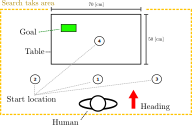
\includegraphics[width=0.8\textwidth]{./ch3-Search/Figures/experimentsetup}
  \caption{Table search task. Blindfolded human subjects after a disorientation step are placed in one of the 
  four starting locations. The heading of the subject is always kept the same. The human's objective is to locate
  the green block on the table. Throughout all experiments the green wooden block is kept in the same location.}
  \label{fig:tab_search_task}
\end{figure}
\begin{figure}
\centering
  \includegraphics[width=\textwidth]{./ch3-Search/Figures/Figure2}
  \caption{\textit{Top left}: A participant is trying to locate the green wooden block on the table
given that both vision and hearing senses have been inhibited. The location of his hand is being tracked by the
OptiTrack\textsuperscript{\textregistered} system. \textit{Top right:} Initial distribution of the uncertainty or belief we assume
the human has with respect to his position. \textit{Bottom left:} Set of recorded searches, the trajectories are with respect to the hand.
\textit{Bottom right:} Trajectories starting from same area but have different search patterns, the red trajectories all navigate to the goal
via the top right corner as opposed to the blue which go by the bottom left and right corner. Among these two groups there are trajectories which
seem to minimize the distance taken to reach the goal as opposed to some which seek to stay close to the edge and corners.}
\label{fig:experiment}
\end{figure}


As covered in the background section, previous work has taken a probabilistic Bayesian approach to model the beliefs and intent 
of humans. A key finding was that humans update their beliefs using Bayes rule (shown so far in the discrete case). 
We make a similar assumption and represent the human's location belief (where he thinks he is) by a particle filter which
is a point mass representation of a probability density function. There is no way of
knowing the human's belief with certainty. We make the critical assumption that the belief is observable in the first time step of the search and all following beliefs 
are assumed correct through applying Bayes integration.
The belief is always initialized to be uniformly distributed on top of the table, 
see Figure \ref{fig:experiment} (\textit{top right}), and the starting position of the human's hand is always in this area.

Before each trial the participant was told that he/she would always be facing the same direction with respect to the table (so always facing the goal, 
like in the case of a door) but his/her translational starting position would vary. 
For instance, the table might not be always directly in front of the person and his/her distance to the edge or 
corner could be varied. In Figure \ref{fig:experiment}
\textit{bottom left}, we illustrate four representative recorded searches whilst in the \textit{bottom right}, we illustrate a set of trajectories 
which all started from the same region. One interesting aspect is the diversity present,
demonstrating clearly that humans behave differently given the same situation.  

It is non-trivial to have a robot learn the behaviour exhibited by humans performing this task. As we cannot encapsulate the true complexity of 
human thinking, we model the human's state through two variables, namely, the human's uncertainty about his current location and the human's  
belief of his position. The various strategies adopted by humans are modelled by building a mapping from the state variables to actions, which are the motion of 
the human arm. Aside from the problem of correctly approximating the belief and its evolution over time, the model needs to take into consideration
that people behave very differently given the same situation. As a result it is not just a single strategy that will be transferred but rather a mixture 
of strategies. 


\section{Formulation} \label{ch3:formulation}

In the standard PbD formulation of this problem, a parametrised function is learned,
mapping from state $x_t$, which denotes the current position of the demonstrator's hand, to  
the hand's displacement $\dot{x}_t$. In our case since the environment is partially observable 
we have a belief or probability density function, $p(x_{t}|y_{0:t},\dot{x}_{1:t})$, which is conditioned on all 
sensing information, $y_{0:t}$, (the subscript, $0:t$, indicates the time slice which ranges from, $t=0$, to 
the current time, $t=t$) over the state space at any given point in time and the history of applied actions, $\dot{x}_{1:t}$. 
We seek to learn this mapping, ${f : p(x_{t}|y_{0:t},\dot{x}_{1:t}) \mapsto \dot{x}_{t+1}}$, from demonstrations. During 
each demonstration we record the following variables:

\begin{itemize}
 \item $\dot{x} \in \mathbb{R}^{3}$, normalised Cartesian velocity of the hand.
 \item $\hat{x} = \argmaxA\limits_{x_t} p(x_{t}|y_{0:t},\dot{x}_{1:t})$, end-effector's most likely position.
 \item $U \in \mathbb{R}$, entropy $H\left(p(x_{t}|y_{0:t},\dot{x}_{1:t})\right)$.
\end{itemize}
We define the belief state to be the compressed vector $b \in \mathbb{R}^4$,

\begin{equation}
 b = \begin{bmatrix}
       \hat{x} \\[0.3em]
       U       \\[0.3em]
     \end{bmatrix}
\end{equation}


A statistical controller was learned from a dataset of $N$ demonstrations: ${\mathcal{D} = \{(\dot{x}^{[i]}_{1:T},b^{[i]}_{1:T})\}_{i=1:N}}$, where the upper index $[i]$
referenced the $i$th search trajectory, recorded during the search trials of the human subjects. Having described the experiment we proceed to give an in-depth description 
of the mathematical representation of the belief, sensing and motion models and the uncertainty. 


\subsubsection{Belief model}


A human's belief of his location in an environment can be multi-modal or uni-modal, Gaussian or non-Gaussian and may change from one distribution to another. 
We chose a particle filter to be able to represent such a wide range of probability distributions. A particle filter is a Bayesian probabilistic method 
which recursively integrates motion and sensing to estimate a posterior from a prior probability density. The particle filter is comprised of two models.
The first, the \textit{motion model} $p(x_{t}|x_{t-1},\dot{x}_{t})$ estimates a distribution over the next possible states. The second, \textit{sensing model} 
$p(y_{t}|x_{t})$, corrects the motion updated distribution through integrating sensing information. These two models are recursively applied and achieve a Bayesian filter in which a prior distribution 
over the state space is turned into a posterior distribution. The two steps are formalised below.

\begin{eqnarray}
 p(x_{t}|y_{0:t-1},\dot{x}_{1:t}) &=& \int p(x_{t}|x_{t-1},\dot{x}_{t})\,p(x_{t-1}|y_{0:t-1},\dot{x}_{1:t-1})\,dx_{t-1} \\
 p(x_{t}|y_{0:t},\dot{x}_{1:t}) &=& \frac{p(y_{t}|x_{t})p(x_{t}|y_{0:t-1},\dot{x}_{1:t})}{p(y_{t}|y_{0:t-1})}
\end{eqnarray}

The probability distribution over the state $p(x_{t}|y_{0:t},\dot{x}_{1:t})$ is represented by a set of weighted particles which represent hypothetical
locations of the end-effector and  their density which is proportional to the likelihood. The particular particle filter used was the 
\textit{Regularised Sequential Importance Sampling} \cite[p.182]{Arul_Mask_Clap_2002}. From previous literature \cite{Bake_Saxe_Tene_2011} 
it has been shown that there is a similarity between Bayes update rule and the way humans integrate information over time. Under this assumption 
we hypothesise that if the initial belief of the human is known then the successive update steps of the particle filter should correspond to a good approximation 
of the next beliefs. 

\subsubsection{Sensing model}

The sensing model gives the likelihood, $p(y_t|x_t)$, of a particular sensation $y_t$ given
a position $x_t \in \mathbb{R}^{3}$. In a human's case, the sensation of a curvature indicates the 
likelihood of being near an edge or a corner. However the likelihood cannot be modelled using 
the human's sensing information. Direct access to pressure, temperature and such salient information is not available. 
Real sensory information needs to be matched against virtual sensation at each hypothetical location $x_t$ of a particle. 
Additionally,  for the transfer of behaviour from human to robot to be successful, the robot should be
able to perceive the same information as the human, given the same situation. An approximation of what a human or robot senses 
can be inferred, based on the end-effector's distance to particular features in the environment. In our case four main features 
are present, namely corners, edges, surfaces and an additional dummy feature defining no contact, air. The choice of these features is prior knowledge 
given to our system and not extracted through statistical analysis of recorded trajectories. The sensing vector is $y_t = \left[p_c,p_e,p_s,p_a\right]^{\mathrm{T}}$, 
is a categorical distribution and prior to normalisation $p$ is the probability of a feature being sensed and the subscript corresponds to 
the first letter of the feature it is associated with. In Equation \ref{eq:sensingfunction}, 
the sensing function, $h(x_t,x_c)$, returns the probability of sensing a corner, where $x_c \in \mathbb{R}^3$ is the Cartesian position of the corner which is
the closest to $x_t$. 

\begin{equation}\label{eq:sensingfunction}
  p_c = h(x_t,x_c;\beta) = \exp\left( -\left(\beta \cdot \|x_t - x_c\|\right)^2 \right)
\end{equation}

The exponential form of the function, $h$, allows the range of the sensor to be reduced. We set $\beta > 0$ such that 
any feature which is more than 1cm way from the end effector or hand has a probability close to zero of being sensed. 
The same sensing function is repeated for all feature types.

The sensing model takes into account the inherent uncertainty of the sensing function \ref{eq:sensingfunction}, 
and gives the likelihood, $p(y_t|x_t)$ of a position. Since the range of sensing is extremely small and entries are probabilistic 
we assume no noise in the sensor measurement.
The likelihood of a hypothetical location $x_t$ is proportional to the Jensen-Shannon divergence (JSD) $p(y_t|x_t) = 1 - JSD(y_t||\hat{y}_t)$ between true sensing vector
$y_t$ obtained by the agent and that of the hypothetical sensation $\hat{y}_t$ generated at the location of a particle. In Figure \ref{fig:pf_example}, four 
different beliefs are shown.

\begin{figure}
  \centering
  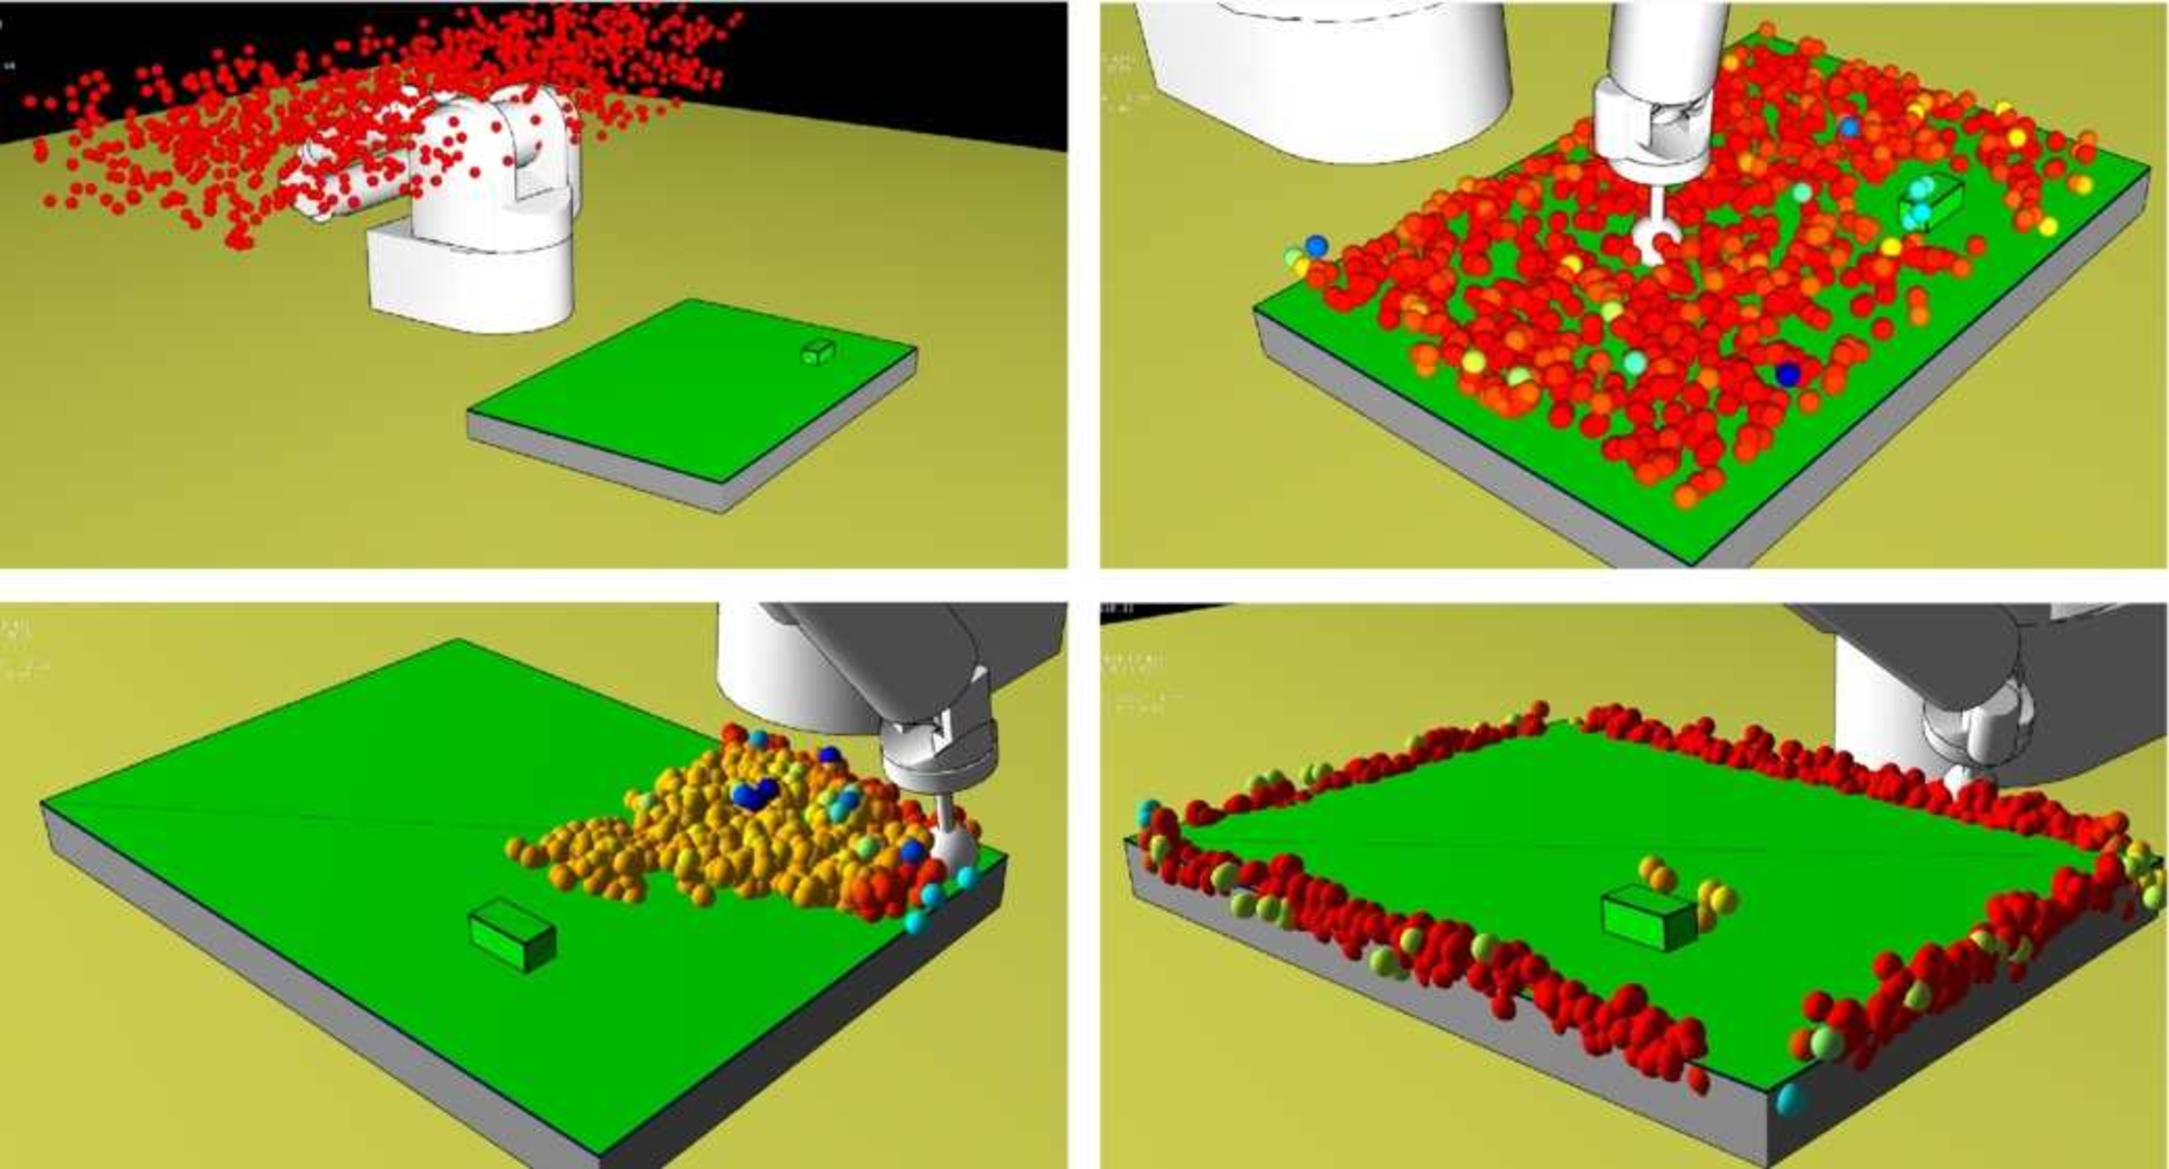
\includegraphics[width=\textwidth]{./ch3-Search/Figures/particlefilter.pdf}
  \caption{Four different time frames of the evolution of the belief particle filter. \textit{Top left}: Initial belief distribution; a lot of uncertainty.
  \textit{Top right:} First contact is made with the table, the measurement likelihood restrains the samples to be on the table's surface. \textit{Bottom right:}
  First contact is an edge. \textit{Bottom left:} Gradual localisation.}
  \label{fig:pf_example}
\end{figure}

\subsubsection{Motion model}

The motion model is straight forward compared with the sensing model. In the robot's case the Jacobian gives the next 
Cartesian position given the current joint angles and angular velocity of the robot's joints.
From this the motion model is given by $ p(x_{t}|x_{t-1},\dot{x}_{t}) = \mathrm{J}(q)\dot{q} + \epsilon$ where $q$ is 
the angular position of the robot's joints, $J(q)$ is the Jacobian and $\epsilon \sim \mathcal{N}(0,\sigma^{2}I)$ is white noise. 
The robot's motion is very precise and its noise variance is very low. For humans, the motion model is the velocity of the hand 
movement provided by the tracking system. In our experiment we consider the noise from motion to be negligible. An increase in 
uncertainty already results from the re-sampling stage of Sampling Importance Resampling (SIR) particle filter and we found 
no need to add additional motion noise.
The particles' positions were updated by applying the measured velocity obtained from either the visual tracking system 
(when recording the human demonstrations) or the robot's forward kinematics.

\subsubsection{Uncertainty}

% First motivate entropy as a natural method for computing the uncertainty

In a probability distribution framework, entropy is used to represent uncertainty. It is the expectation of a 
random variable's total amount of unpredictability. The higher the entropy the more the uncertainty, likewise the 
lower the entropy, the less the uncertainty. In our context, a set of weighted samples replaces 
the true probability density function of the belief, $p_{\Param}(x_t|y_{0:t},\dot{x}_{1:t})$. A reconstruction of 
the underlying probability density is achieved by fitting a Gaussian  Mixture Model (GMM), Equation \ref{eq:gmm1}, to the particles,

\begin{equation}\label{eq:gmm1}
  p_{\Param_H}(x_t|y_{0:t},\dot{x}_{1:t}) = \sum\limits_{k=1}^{K} \piK\, g(x_t\: ;\MuK,\SigK )
\end{equation}
where parameters $\Param_H = \{w^{[k]},\MuK,\SigK\}_{1:K}$, are the weights, means and covariances of the individual multivariate Gaussian function, $g(\cdot)$ and
$K$ is the number of Gaussian components. The scalar $\piK$ represents the weight associated to mixture component $k$ 
(indicating the component's overall contribution to the distribution) and $\sum_{k=1}^{K} \piK = 1$. The parameters $\MuK \in \mathbb{R}^{(3\times 1)}$ 
and $\SigK \in \mathbb{R}^{(3\times 3)}$ are the mean and covariance of the normal distribution $k$. 

The main difficulty here is determining the number of parameters of the density function in a computationally efficient manner.
We approach this problem by finding all the modes in the particle set via mean-shift hill climbing and set these as the 
means of the Gaussian functions. Their covariances are determined by maximizing the likelihood of the density function 
via Expectation-Maximization (EM). 
%
%	images/clustering.eps
%

\begin{figure}
 \centering
   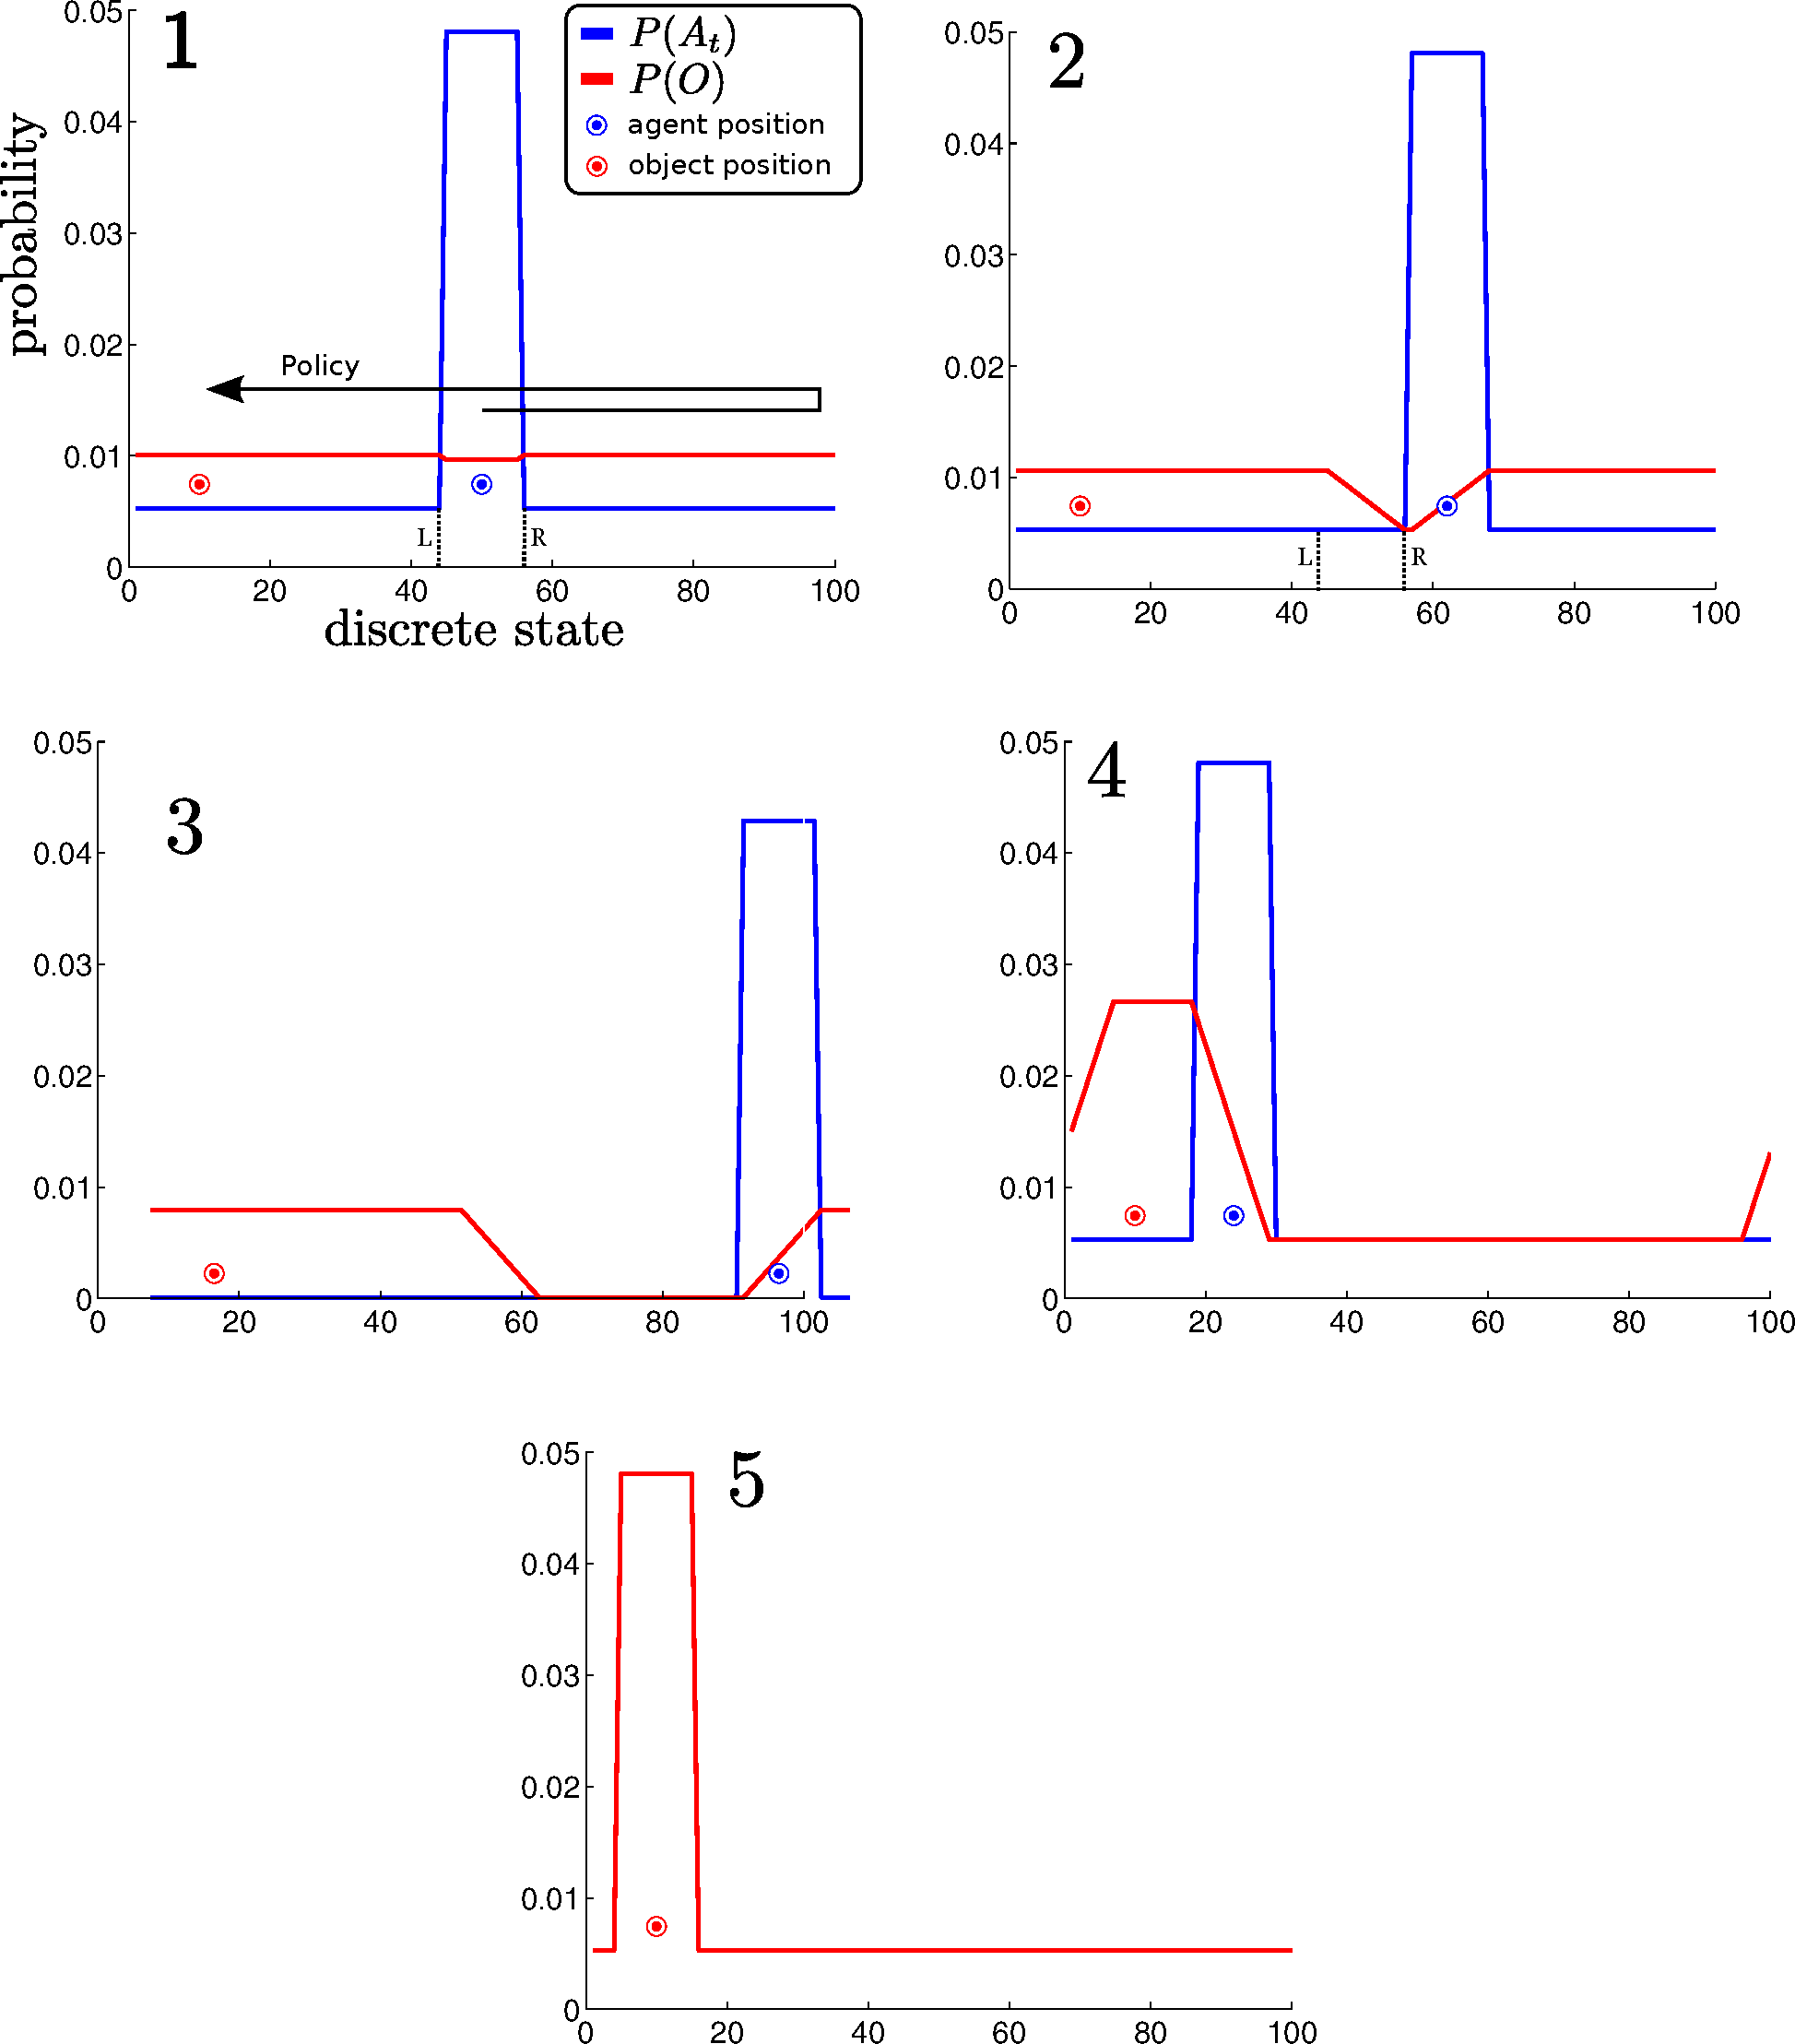
\includegraphics[width=0.95\textwidth]{./ch3-Search/Figures/Figure3}
  \caption{Representation of the estimated density function $p_{\Param_H}(x_t|y_{0:t},\dot{x}_{1:t})$. \textit{Top Left and Right:} Initial starting point, 
  all Gaussian functions are uniformly distributed with uniform priors. The red cluster always has the highest likelihood which is taken
  to be the believed location of the robot's/human's end-effector. \textit{Bottom Left:} Contact with the table has been established, the robot location differers
  from his belief. \textit{Bottom Right:} Contact has been made with a corner, the clusters reflect that the robot could be at any corner (note that weights are not 
  depicted, only cluster assignment).}
  \label{fig:clustering}
\end{figure}

Given the estimated density we can compute the upper bound of the differential entropy $H(\cdot)$ \citep{DiffEntropyHuber2008},
%which is taken to be the uncertainty $U$,
\begin{equation}
  H\left(  p_{\Param_H}(x_t|y_{0:t},\dot{x}_{1:t}) \right) = \sum\limits_{k=1}^{K} \piK\ \left( -\log(\piK) + \frac{1}{2} \log((2\pi e)^{D} |\Sigma_{k}|) \right)
\end{equation}
where $e$ is the base of the natural logarithm and $D$ the dimension (being 3 in our case).

The reason for using the upper bound is that the exact differential entropy of a mixture of Gaussian functions has no 
analytical solution. When computing both the
upper and lower bounds it was found that the difference between the two was insignificant, making any bound a good approximation 
of the true entropy. The choice of the believed location of the robot/human end-effector is taken to be the mean of the 
Gaussian function with the highest weighted $w$.

\begin{equation}
 \hat{x}_t = \operatorname*{arg\,max}_{x_t} p_{\Param_H}(x_{t}|y_{0:t},\dot{x}_{1:t}) = \Mu{\argmaxA\limits_{k}(w^{[k]})}
\end{equation}

Figure \ref{fig:clustering} depicts different configurations of the modes (clusters) and believed position of the end-effector (indicated by a yellow arrow).  



%%%%%%%%%%%%%%%%%%%%%%%%%%%%%%%%%%%%%%%%%%%%%%%%%%%%%%%%%%%%%%%%%%%%%%%%%%%%%%%%%%%%%%%%%%%%%%%%%%%%%%%%%%%%%%%%%%%%%%%%%%%%%%%%%%%%%%%%%
%																	   %
%					Methods												   %
%																	   %
%%%%%%%%%%%%%%%%%%%%%%%%%%%%%%%%%%%%%%%%%%%%%%%%%%%%%%%%%%%%%%%%%%%%%%%%%%%%%%%%%%%%%%%%%%%%%%%%%%%%%%%%%%%%%%%%%%%%%%%%%%%%%%%%%%%%%%%%%


\section{Policies}\label{chap3:policies}

\subsection{Modelling human search strategies}\label{chap3:GMM_policy}

During the experiments, the recorded trajectories show that different actions are present for the same belief and uncertainty making the data multi-modal
(for a particular position and uncertainty different velocities are present). That is multiple actions are possible given a specific belief. 
This results in a one-to-many mapping which is not a valid function, eliminating any regression technique which directly learns a non-linear function. 
To accommodate this fact we use a GMM to model the human's demonstrated searches. Using statistical models to encode control policies in robotics is quite common, see \cite{Billard08chapter}. 

% explain how much data we have vs the number of gaussian components
By normalising the velocity the amount of information to be learned was reduced. We also took into consideration that velocity is more 
specific to embodiment capabilities: the robot might not be able to reproduce safely some of the velocity profiles demonstrated. 

The training data set comprised a total of 20'000 tuples $(\U,\B)$, from the 150 trajectories gathered from the demonstrators. 
The learned GMM $\pi_{\Param}(\U,\B)$ had a total of 7 dimensions, $\U \in \mathbb{R}^3$ and $\B \in \mathbb{R}^4$. 
The definition of the GMM is presented below in Equation \ref{eq:gmm2}.

\begin{equation} \label{eq:gmm2}
 \pi_{\Param}(\U,\B) = \sum\limits_{k=1}^{K} \piK \, g(\U,\B;\MuK,\SigK) 
\end{equation}
The parameters $\Param = \{w^{[k]},\MuK,\SigK\}_{1:K}$, are the weights, means and covariances 
of the individual Gaussian functions, $g(.)$,
\begin{center}
$\MuK =  \begin{bmatrix} \MuK_{\U} \\ \MuK_{\B} \end{bmatrix}$, 
$\SigK =  \begin{bmatrix} 
	  \SigK_{\U\U} & \SigK_{\U\B} \\
	  \SigK_{\B\U} & \SigK_{\B\B}
	  \end{bmatrix}$
\end{center}
where $\sum_{k} w^{[k]} = 1$, $\MuK_{\U} \in \mathbb{R}^{3}$ and  $\MuK_{\B} \in \mathbb{R}^{4}$. Given this generative representation of the humans' demonstrated searches we proceeded to 
select the necessary parameters to correctly represent the data. This step is know as model selection and we used Bayesian Information Criterion (BIC) to evaluate
each set of parameters which were optimised via Expectation-Maximisation (EM). 

A total of 82 Gaussian functions were used in the final model, 67 for trajectories on the table and 15 for those in the air. In Figure
\ref{fig:gmm} \textit{(left)} we illustrate the model learned from human demonstrations where we plot the 3 dimensional slice (the position) of the 7
dimensional GMM to give a sense of the size of the model.

\begin{figure}
\centering
  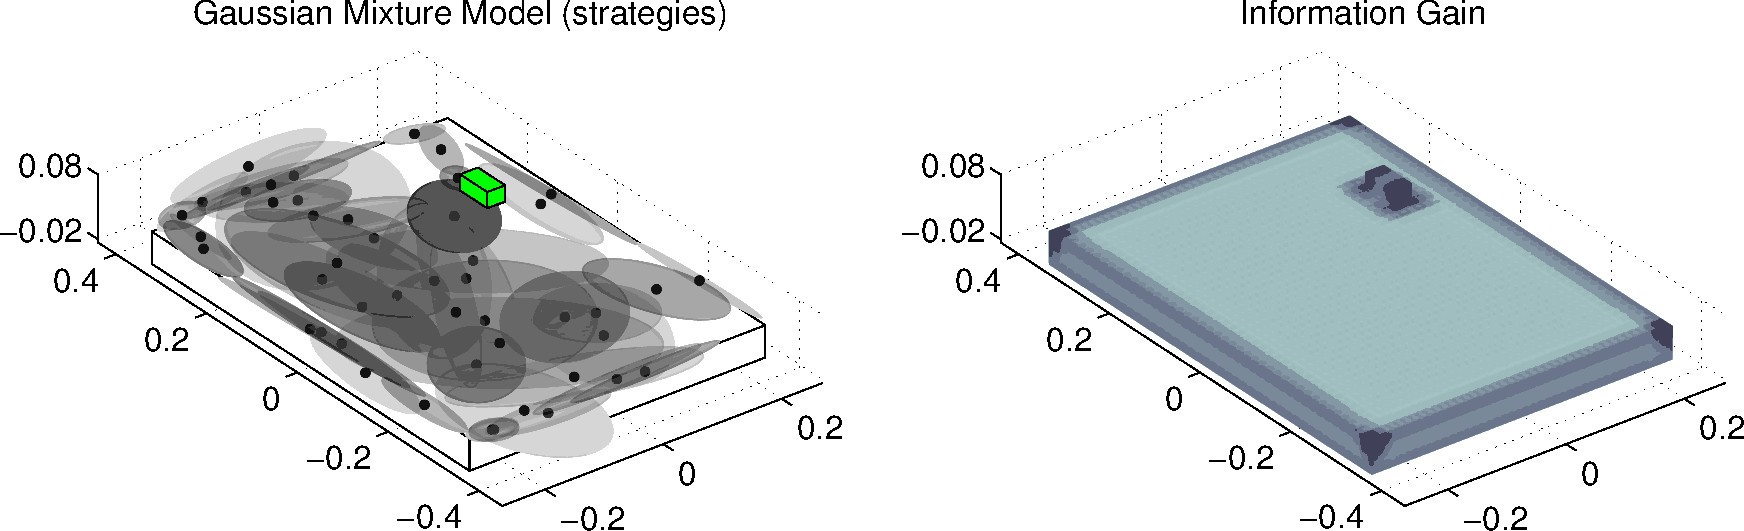
\includegraphics[width=0.95\textwidth]{./ch3-Search/Figures/Figure4}
  \caption{\textit{Left: } Resulting search GMM, a total of 67 Gaussian mixture components are present. We note the many overlapping Gaussians: this results
from the level of uncertainty over the different choices taken. For example humans follow along the edge of the table in different directions and might
leave the edge once they are confident with respect to their location. \textit{Right:} Information Gain map ($I(x)$ Equation \ref{eq:IG}) of the table environment, dark regions indicate 
high information gain as oppose to lighter ones. Not surprisingly, the highest are the corners, followed by the edges.}
  \label{fig:gmm}
\end{figure}

\subsection{Coastal Navigation}\label{chap3:costal_policy}

Coastal navigation \citep{CostalNavigation1999} is a path planning method in which the objective function, 
Equation \ref{eq:objective_function}, is composed of two terms.

\begin{equation}\label{eq:objective_function}
 f(x_{0:T}) = \sum\limits_{t=0}^{T} \lambda_1 \, c(x_t) + \lambda_2 \, I(x_t)
\end{equation}

The first term $c(x_t)$ is the traditional ``cost to go'' which penalizes every step taken so as to ensure that the
optimal path is the shortest. The value was simply set to 1 for all discrete states in our case. The second term, $I(x_t)$, 
is the information gain of a state. The information gain of a particular state is related to how much 
the entropy of a probability density function (pdf), being the location's uncertainty in our case, can be reduced. The two $\lambda$'s are scalars which weigh the influence 
of each term. There is no constraint that they must sum to one.

In our table environment we discretised the state space, $\mathbb{R}^3$, into bins so as to have a resolution of approximately, $1\, cm^3$, giving us a total of a 125'000
states. The action space was discretised to 6 actions, two for each dimension meaning that all motion is parallel to the axis. For each state $x$ an $I(x)$ value is
computed by evaluating Equation \ref{eq:IG},

% Explain how the Information Gain is computed

\begin{equation}\label{eq:IG}
 I(x) = \mathbb{E}_{p(y_t|x_t)}\{ H(p_{\Param_H}(x_t|y_{0:t},\dot{x}_{1:t}) \} - H(p_{\Param_H}(x_t|y_{0:t-1},\dot{x}_{1:t}))
\end{equation}
which is essentially the difference between the entropy of a prior pdf to that of a posterior pdf.
We set our initial pdf to be uniformly distributed and  we computed the maximum likelihood sensation for each discrete state $x_t$
which is akin to the expected sensation or assuming that there is no uncertainty in sensor measurement (an assumption 
often made throughout the literature to avoid carrying out the integral of the expectation in Equation \ref{eq:IG}).
The result is the difference between the posterior pdf, given that the sensation occurred in $x_t$, and the prior pdf. The resulting cost
map is illustrated in Figure \ref{fig:gmm}. As expected, corners have the highest information gain followed by edges and surfaces. 
We do not show the values above the table since they provided much less information gain.

The optimization of the objective function is accomplished by running the Dijkstra's algorithm. This algorithm, given a cost map, 
computes the shortest path to a specific target from all the states. This results in a policy.

\subsection{Control}\label{sub:ch3:control}
The standard approach to control with a GMM is to condition on the belief state $b$ and perform inference on the resulting conditional
GMM, Equation \ref{eq:conditional}, which is a distribution over velocities or directions.

\begin{equation} \label{eq:conditional}
  \pi_{\Param}(\U|\B) = \sum\limits_{k=1}^{K} w^{[k]}_{\U|\B} \;\;  g\left(\U\: ;  \MuK_{\U|\B}, \SigK_{\U|\B} \right)
\end{equation}

The new distribution is of the dimension of the output variable, the velocity (3 dimensions). 
The variable $\U$ in $\U|\B$ indicates the predictor variable and the variables $\B$ has been conditioned.
A common approach in statistical PbD methods using GMMs is to take the expectation of the conditional (known as Gaussian Mixture Regression), Equation \ref{eq:GMR}

\begin{equation} \label{eq:GMR}
 \dot{x} = \mathbb{E}\{\pi_{\Param}(\dot{x}|\B)\} = \sum\limits_{k=1}^{K}  w^{[k]}_{\dot{x}|\B} \; \MuK_{\U|\B}
\end{equation}

The problem with this expectation approach, is that it averages out opposing directions or strategies and may result in 
a net velocity of zero. One possibility would be to sample from the conditional, however this can lead to non-smooth 
behaviour and flipping back and forth between modes resulting in no displacement. To maintain consistency between the
choices and avoid random switching  we perform a weighted expectation on the means so that 
directions (modes) similar to the current direction of the end-effector receive
a higher weight than opposing directions. For every mixture component $k$, a weight $\alpha_k$ is computed based 
on the distance between the current direction and itself.
If the current direction agrees with the mode then the weight remains unchanged but if it is in
disagreement a lower weight is
calculated according to the equation below. 
\begin{equation}  \label{eq:weight}
  \alpha_{k}(\U) = \piK_{\U|\B} \; \exp(-\cos^{-1}(<\U,\MuK_{\U|\B}>))
\end{equation}
Gaussian Mixture Regression is then performed with the normalised  weights $\alpha$ instead of $wi$
(the initial weight obtained when conditioning).

\begin{equation}\label{eq:w_expectation}
 \underline{\U} = \mathbb{E}_{\alpha}\{\pi_{\Param}(\U|\B)\} = \sum\limits_{k=1}^{K} \alpha_{k}(\U) \:\MuK_{\U|\B}
\end{equation}
% 
%	How to control speed
%
The final output of Equation \ref{eq:w_expectation} gives the desired direction
($\U$ is re-normalised and is denoted as $\underline{\dot{x}}$). In the case when the mode suddenly disappears
(because of sudden change of the level of uncertainty caused by the appearance or disappearance of a feature)
another present mode is selected at random. For example, when the robot has reached a corner, the level of uncertainty for this feature drops to zero.
A new mode, and hence new direction of motion, will then  be computed.
However this is not enough to be able to safely control the robot.
One needs to control the amplitude of the velocity and ensure compliant control 
of the end-effector when in contact with the table. This behaviour is not learned here, as this is specific to 
the embodiment of the robot and unrelated to the search strategy. The 
amplitude of the velocity is computed by a proportional controller based on the
believed distance to the goal,
\begin{align} \label{eq:ch3:amplitude}
     \nu &= \max(\min(\beta_{1},K_{p}(x_{\mathrm{g}} - \hat{x}),\beta_{2}) \\ \nonumber
 \dot{x} &=  \nu\,\underline{\dot{x}}
\end{align}
where the $\beta$'s are lower and upper amplitude limits, $x_{g}$ is the
position of the goal, and $K_{p}$ the proportional gain which was tuned through
trials.

%
%	images/flow_chart.eps
%

\begin{figure}
 \centering
 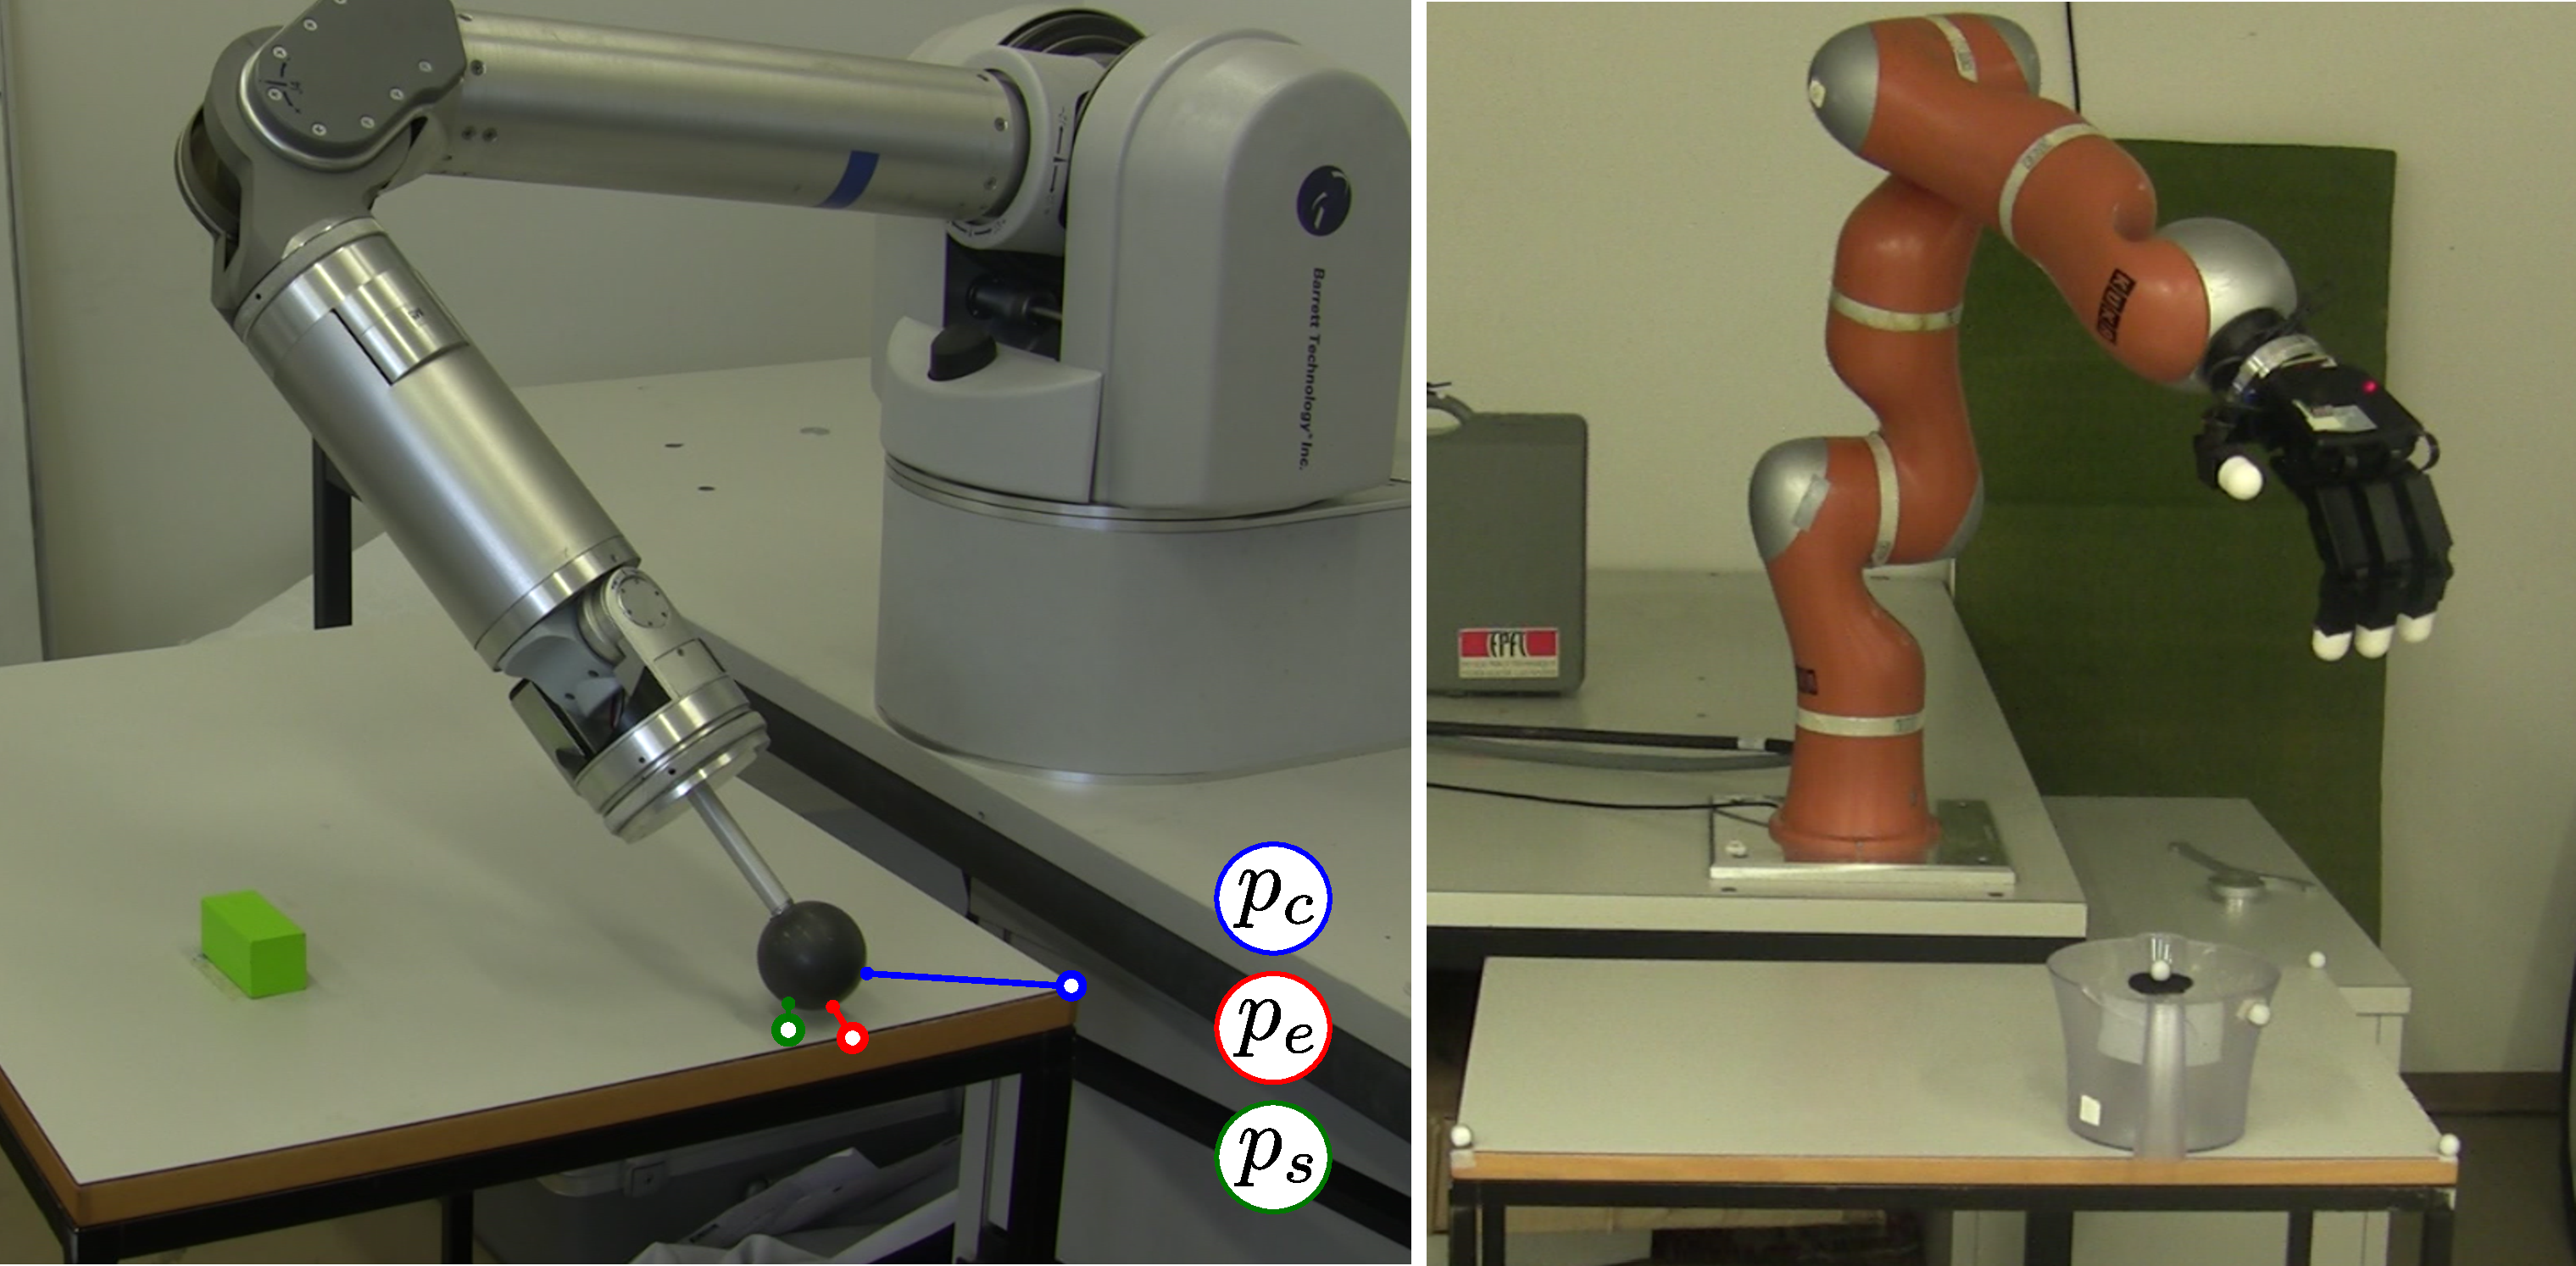
\includegraphics[width=\textwidth]{./ch3-Search/Figures/robots}
 \caption{\textit{Left:} The WAM is cable driven 7 Degrees of Freedom (DOF) robot and is controlled by directly sending torque commands. 
 \textit{Right}: The KUKA LWR is as the WAM a 7 (DoF) robot. Both robots are controlled via an Ethernet cable at a 1kHz communication rate. The KUKA API 
 provides a command interface to the stiffness, damping, position and torque variables of each joint in contrast to the WAM for which our own impedance 
 controller was developed. In our setup the end-effector of the WAM is a haptic device from which we computed sensations $y$, by treating it as a point mass with respect
 to the model of the world and use Equation \ref{eq:sensingfunction} on page \pageref{eq:sensingfunction} to compute the measurements. The KUKA is equipped 
 with the Allegro hand from which we compute sensations from each finger tip, also by considering geometric distances with features in the environment.}
 \label{fig:ch3:wam:kuka}
\end{figure}

\subsection{Robot implementation}

The above procedure can control the general behaviour of the search but is insufficient for a successful implementation on a robotic system 
such as the 7 Degree of Freedom $q\in\mathbb{R}^7$ ($q$ is a vector of joint positions) WAM or KUKA LWR robot, which we illustrate in Figure \ref{fig:ch3:wam:kuka}. 
The GMM policy $\underline{\dot{x}} = \mathbb{E}_{\alpha}\{\pi_{\Param}(\dot{x}|b)\}$ outputs a linear velocity and the 
angular velocity is computed from a reference orientation which is constant. 
From both linear and angular velocities a reference position $x^r \in \mathbb{R}^{(3 \times 1)}$ and orientation $R^r \in \mathbb{R}^{(3 \times 3)}$ are computed and used to 
define a linear and angular error $x_e = x^r - x$, $\psi_e = \mathrm{angleaxis}(R^{\mathrm{T}}R^r)$ by using the  
the current position $x$ and orientation $R$ of the robot's end-effector.
Given the kinematic chain of the robot, the inverse of the Jacobian $J(q) \in \mathbb{R}^{6\times 7}$ is used in an impedance control to transform the 
Cartesian error $c_e = [x_e,\psi_e]^{\mathrm{T}} \in \mathbb{R}^{6 \times 1}$ to torque commands $\tau_t \in \mathbb{R}^7$, Equation \ref{eq:ch3:torque_control},

\begin{equation}\label{eq:ch3:torque_control}
 \tau_t = J^{\mathrm{T}}(q_t)\left(-K c_e - D \dot{c}_e \right) + g(q_t)
\end{equation}

where $K,D \in \mathbb{R}^{6\times6}$ are diagonal stiffness and damping matrices whose values were set experimentally 
and $g(q_t)$ compensates for gravity. Given an applied torque there is a resulting joint velocity $\dot{q}_t$ from which we can compute the 
measured Cartesian end-effector velocity used in the motion model of the particle filter. The learned search strategies were evaluated both on 
the WAM and KUKA illustrated in Figure \ref{fig:ch3:wam:kuka}. Figure \ref{fig:ch3:control_flow} illustrates the complete control flow.

\begin{figure}
\centering
  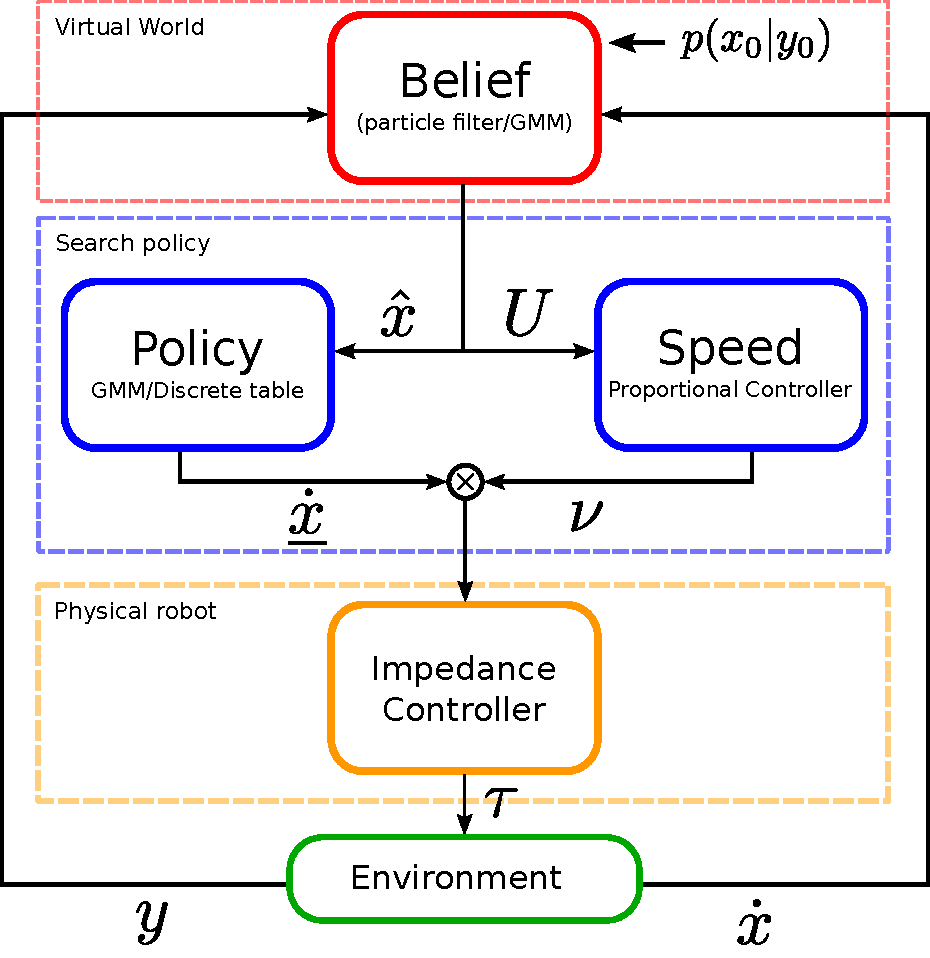
\includegraphics[width=0.8\textwidth]{./ch3-Search/Figures/Control_schematics}
  \caption{Overview of the decision loop. At the top a strategy is chosen given an initial belief
$p(x_{0}|y_{0})$ of the location of the end-effector (initially through sampling the conditional). 
A speed is applied to the given direction based on the believed distance
to the goal. This velocity is passed onwards to
a low level impedance controller which sends out the required torques. The
resulting sensation, encoded through the Multinomial distribution over
  the environment features, and actual displacement are sent back to update the
belief.}
  \label{fig:ch3:control_flow}
\end{figure}
%%%%%%%%%%%%%%%%%%%%%%%%%%%%%%%%%%%%%%%%%%%%%%%%%%%%%%%%%%%%%%%%%%%%%%%%%%%%%%%%%%%%%%%%%%%%%%%%%%%%%%%%%%%%%%%%%%%%%%%%%%%%%%%%%%%%%%%%%
%																	   %
%				Results and Discussion  										   %
%																	   %
%%%%%%%%%%%%%%%%%%%%%%%%%%%%%%%%%%%%%%%%%%%%%%%%%%%%%%%%%%%%%%%%%%%%%%%%%%%%%%%%%%%%%%%%%%%%%%%%%%%%%%%%%%%%%%%%%%%%%%%%%%%%%%%%%%%%%%%%%
\FloatBarrier
\section{Results and discussion}\label{chap3:results}

Throughout our evaluation of our GMM PbD-POMDP control policy we will be considering four search policies: Greedy, GMM, Hybrid and 
Coastal. We evaluate behaviour present in the human demonstrations, and the four above mentioned policies in terms 
of their risk. We qualitatively compare the policies of the GMM model and the Coastal Navigation algorithm and highlight the 
effect of uncertainty. We finish with a quantitative evaluation of search efficiency in terms of distance travelled until the goal is found.
The outline of this section follows as:
\begin{itemize}
 \item Section \ref{sub:search_behaviour}, we analyse the types of behaviour present in the human demonstration as well as in
four different search algorithms: Greedy, GMM, Hybrid and Coastal.
 \item Section \ref{sub:policy_analysis}, we qualitatively analyse the GMM search policy (namely the different modes/decisions present) 
 with respect to the Coastal navigation policy.
 \item Section \ref{sub:time_uncertainty}, we evaluate the search performance, with respect to the distance taken to reach the goal and the uncertainty profiles towards the end of 
the searches in 5 different experiments (different types of initializations). 
\end{itemize}
\FloatBarrier
\subsection{Search \& behaviour analysis}\label{sub:search_behaviour}

For each method (Greedy, GMM, Hybrid, Coastal) 70 searches were performed with all starting positions drawn from the
uniform distribution used during the teaching stage (depicted in Figure \ref{fig:experiment} \textit{top right}, page \pageref{fig:experiment}). 
In Figure \ref{fig:expectedfeatures} we illustrate the expected sensation $\mathbb{E}\{y\}$ and  variance $\mathrm{Var}\{y\}$ for each trajectory with respect 
to the edge and corner of the table. 

\begin{figure}
  \centering
  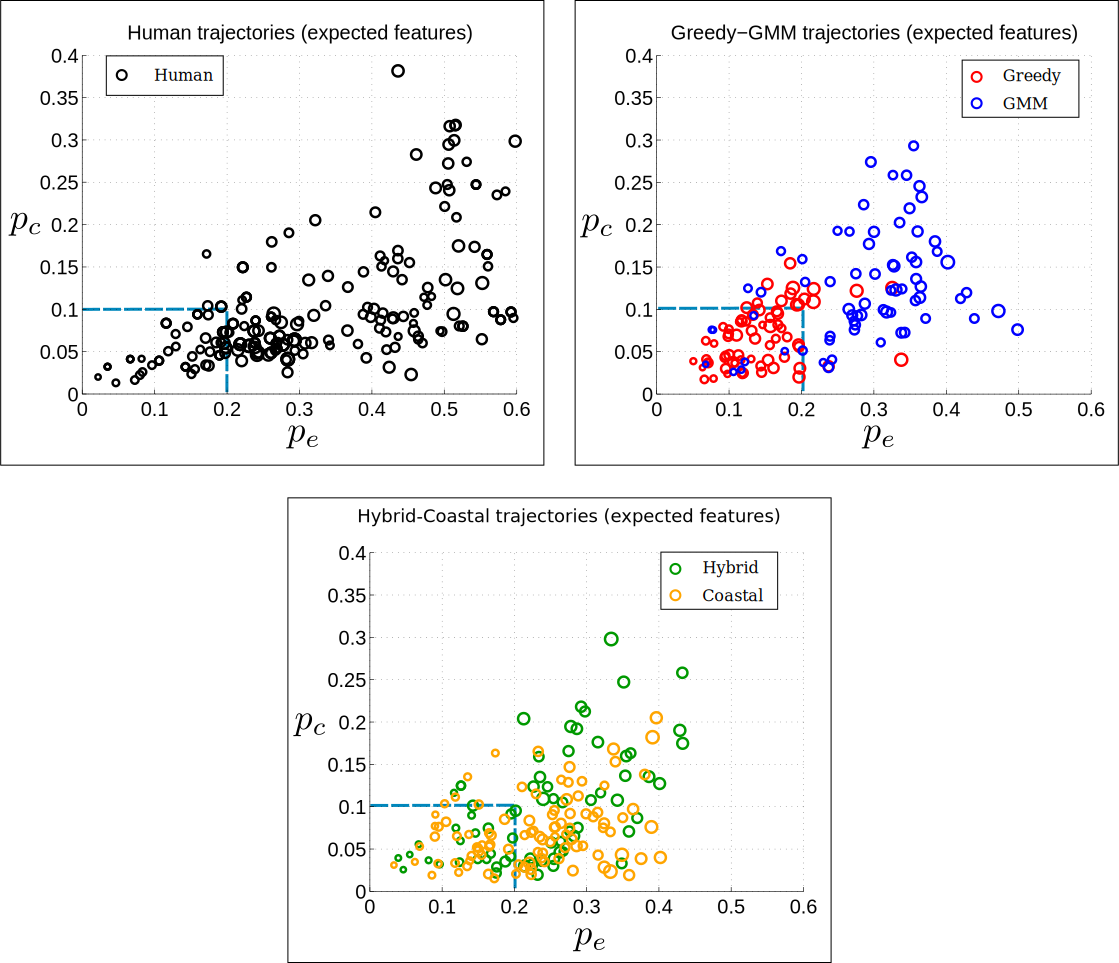
\includegraphics[width=\textwidth]{./ch3-Search/Figures/Figure6} 
  \caption{Expected sensation. Plots of the expected sensation of the edge and corner feature for all trajectories. 
  The axes are associated with the 
  sensor measurements, 0 means that the corresponding feature is not sensed and 1 the feature is fully sensed. 
  A point in the plots summarises a whole trajectory by the mean and variance of the probability of sensing a corner or edge. 
  The radius of the circles are proportional to the variance. The doted blue rectangle represents the decision boundary 
  for classifying a trajectory as being either risk-prone or risk-averse. A point which lies inside the rectangle is risk-prone.
  \textit{Left:} Human trajectories demonstrate a wide variety of behaviours ranging from those remaining close to features 
  to those preferring more risk. 
  \textit{Right:} Red points show Greedy and blue points the GMM model. 
  \textit{Bottom:} Green circles are associated with the Hybrid method whilst orange are those of the 
  Coastal navigation method. The Hybrid method is a skewed version of the GMM which tends towards risky behaviour and exhibits the 
  same kind of behaviour as the Coastal algorithm.}
  \label{fig:expectedfeatures}
\end{figure}


The selection of edges and corners as features as a means of classifying the type of behaviours present 
is not solely restricted to our search task. Salient landmarks will result in a high level of information
gain, which is the case for the edge and corner (see Figure \ref{fig:gmm} \textit{right}, page \pageref{fig:gmm}).
Other tasks can use such features or variants in which the curvature is considered for representing the task space. 
These features are present in most settings and high level features can use these easily as their building blocks.

We note that the Greedy search approach seeks to go directly to the goal without taking into account 
the uncertainty. The GMM models human search strategies. The Hybrid is a combination of both the Greedy and GMM method 
where once the uncertainty has been sufficiently minimised, the policy switches (threshold) to the Greedy method for the rest of 
the search. The Coastal navigation algorithm finds the optimal path to the goal based on an objective function which
consists of a trade-off between time taken to reach the goal and the minimisation of the uncertainty.

It can be seen that the human demonstrations have a much wider spread than those of the search algorithms. 
We speculate that this is due to human behaviours being optimal with respect to their own criteria as opposed to the algorithms 
which usually tend to only maximise a single objective function. The trajectories of the Greedy and GMM methods represented by their 
expected features demonstrate two distinctive behaviours (in terms of expected sensation), risk-prone for the Greedy and risk-adverse
for the GMM.

We make \textbf{the assumption} that Greedy trajectories are risk-prone by nature. We performed a SVM classification on the 
Greedy-GMM expected features (Figure \ref{fig:expectedfeatures} \textit{right}) and used the result to construct a decision boundary as a means
of classifying a trajectory as being either risk-prone or risk-averse. Table \ref{tab:percentage-risk-prone} \textit{first row} shows that
the GMM and Human search trajectories are mostly risk-averse. Surprisingly the Coastal policy seems to be very risk-prone given 
that it seeks paths close to highly informative areas.
We use a second metric based on the information gain, which we call the Risk factor, to classify trajectories as being either 
risk-prone or risk-averse.

The Risk factor of each individual trajectory is inversely proportional to its accumulated information gain. Figure \ref{fig:riskexamples} (\textit{left}) shows the kernel density estimation distribution of the risk 
for each search method. Two trajectories per search type corresponding to a supposed risk-prone and risk-averse search
are plotted in the expected feature space in Figure \ref{fig:riskexamples} (\textit{right}). As expected, risk-prone strategies 
for which the risk tends to 1 have a low expectation of sensing edges and corners and produce trajectories with a 
low information gain while those with a high expectation of sensing features have a high information gain. 
Since the metric lies exclusively in the range [0,1] we define that every trajectory which has a Risk factor lower than than 0.5 will 
be considered risk-averse whilst those above are risk-prone. Table \ref{tab:percentage-risk-prone} \textit{second row} illustrates
the riskiness of each search method. It is evident that humans are risk-averse in general followed by GMM which is a smoothing 
of the human data, then Hybrid which as expected should be more risk-prone since it is a linear interpolation between the GMM and 
Greedy search policies and finally Coastal and Greedy.

\begin{figure}
  \centering
  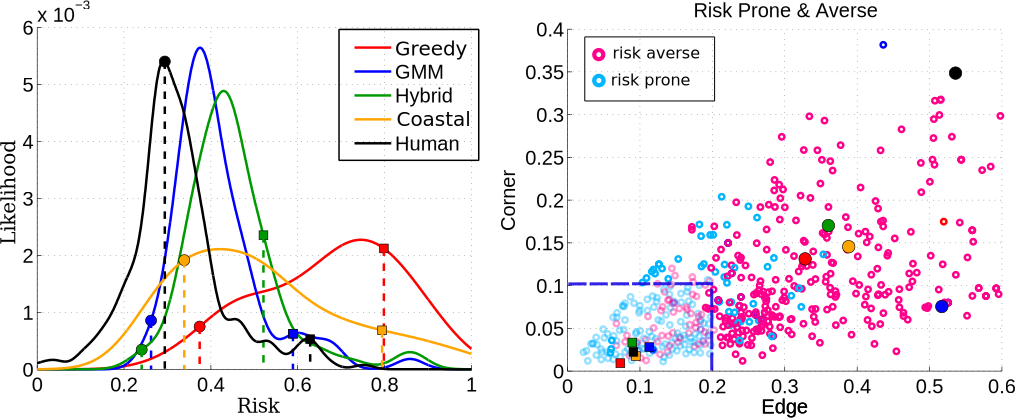
\includegraphics[width=\textwidth]{./ch3-Search/Figures/risk-averse-dist-features} 
 \caption{Risk of searches. Illustration of risk-prone and risk-averse searches in terms of a Risk factor (\textit{left}) and expected sensation (\textit{right}).
 \textit{Left:} Each trajectory was reduced to a single scalar, which we call the Risk factor, quantifying the risk of a trajectory. The Risk factor 
 is inversely proportional to the sum of the information gain of a particular trajectory. The colour paired dots (risk averse) and squares (risk prone) 
 represent trajectories which are plotted in 
 Figure \ref{fig:risk_examples}, to illustrate that these correspond to risk averse and prone searches.
 \textit{Right:} Corresponding trajectories chosen in the Risk factor space but represented in the feature space. As expected, trajectories with
 a high risk map to regions of low expected feature. However the transition from the Risk space to feature space is non-linear and will result in a different
 risk-level classification than the feature metric previously discussed.}
 \label{fig:riskexamples}
\end{figure}



\begin{table}
\centering
\begin{minipage}{\textwidth}
\centering
 \begin{tabular}{|l|c|c|c|c|c|}
 \cline{1-6}
   Criteria        &  \textbf{Greedy} & \textbf{GMM}  & \textbf{Hybrid} & \textbf{Coastal} & \textbf{Human} \\ \hline
  risk-prone (f) &   77 \% & 11 \% &  30 \% & 46 \% & 26  \% \\ \hline
  risk-prone (r) &   78 \% & 12 \% &  24 \% & 45 \% &  7 \% \\ \hline
 \end{tabular}
\end{minipage}
 \caption{Percentage of risk-prone trajectories based on two decision criteria, the feature (f) and the risk (r) (information gain) metrics discussed above.}
 \label{tab:percentage-risk-prone}
\end{table}

Figure \ref{fig:risk_examples} (\textit{top left \& right}), shows risk-prone (red) and 
averse (green) trajectories produced by human demonstrations and by the Greedy search. Both these extremes
correspond to our intuition that risk-averse trajectories tend to remain closer to features or areas of high information gain
as oppose to risk-prone searches. However to stress the case that humans have multiple search strategies 
present, we performed 40 GMM searches (model of the human behaviour) which all started under the same initial conditions
(same belief distribution, true position and believed position). Figure \ref{fig:risk_examples}
shows the resulting trajectories and expected features for each trajectory. 
It is clear that multiple searches occur which is reflected in the plot of the expected features. All of the 
search strategies generated by the GMM for this initial condition produced risk-averse trajectories.


We conclude that there is evidence of multiple search strategies present in the human searches since they were extracted and encoded in the GMM model. 
From the risk distribution, humans have a tendency to be risk-averse.

\begin{figure}
 \centering
  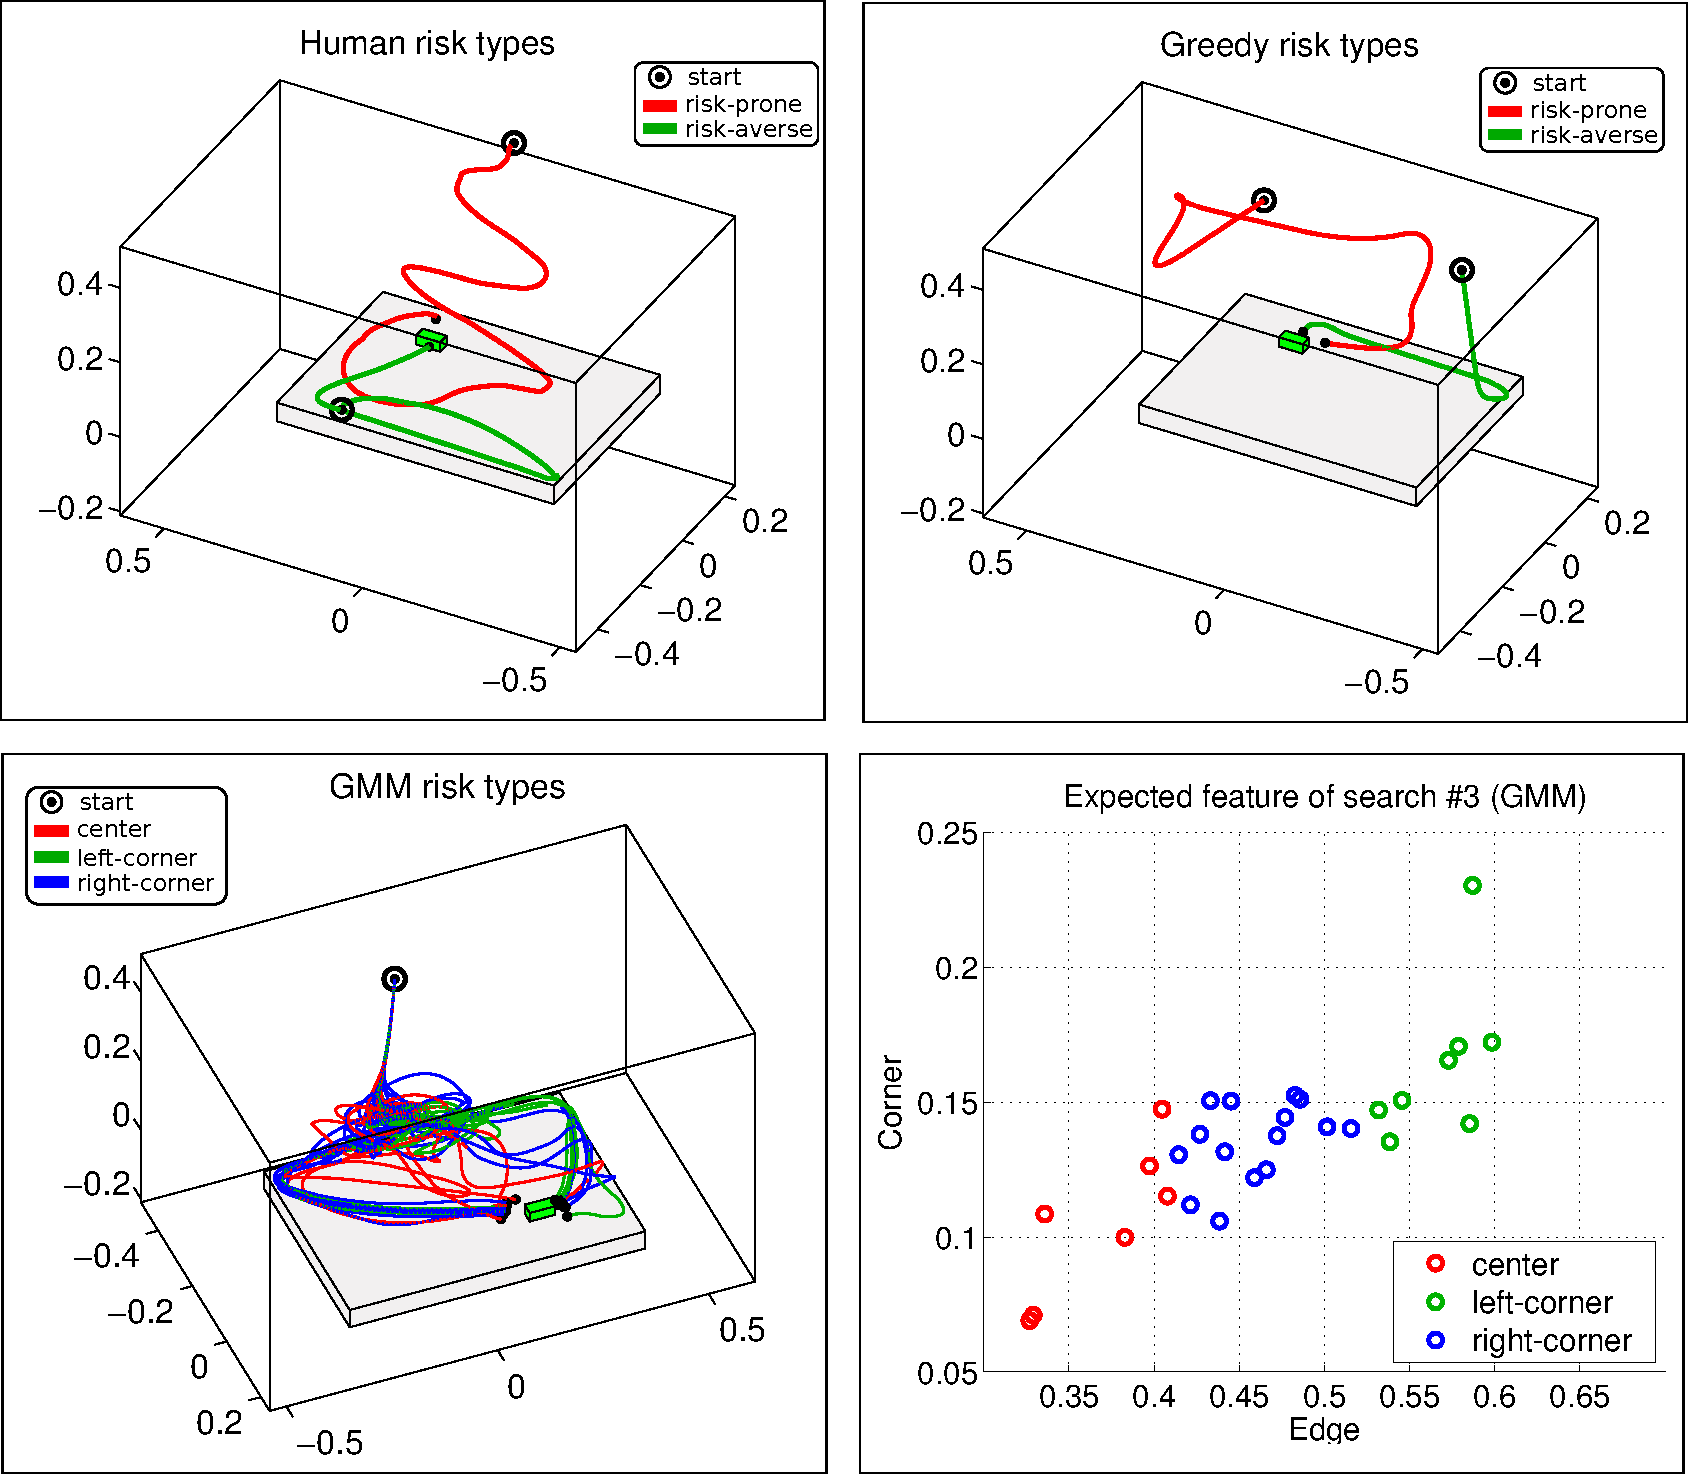
\includegraphics[width=0.95\textwidth]{./ch3-Search/Figures/Figure8}
  \caption{Risk prone \& averse searches (red \& green trajectories). \textit{Top left:}
  Two human trajectories taken from data shown in Figure \ref{fig:riskexamples}. 
  \textit{Top right:} Two Greedy trajectories. \textit{Bottom left:} GMM trajectories, all starting from the same location, the
  colour coding is to illustrate the different policies which were encoded and emerge given the same initial conditions. 
  \textit{Bottom right:} Corresponding expected features of each trajectory, the colour coding matches the trajectories 
  to the ``GMM risk types'' sub-figure. All the searches which were generated by the GMM for this initialisation produced
  risk-averse searches (based on the feature metric discussed previous).}
  \label{fig:risk_examples}
\end{figure}

\FloatBarrier
\subsection{GMM \& Coastal Navigation policy analysis}\label{sub:policy_analysis}

We next illustrate some of the modes (action choices) present during simulation and evaluate their 
plausibility. Figure \ref{fig:modes} shows that multiple decision points have been correctly embedded in the GMM model. All
arrows (red) indicate directions that reduce the level of uncertainty. 

\begin{figure}
    \centering
    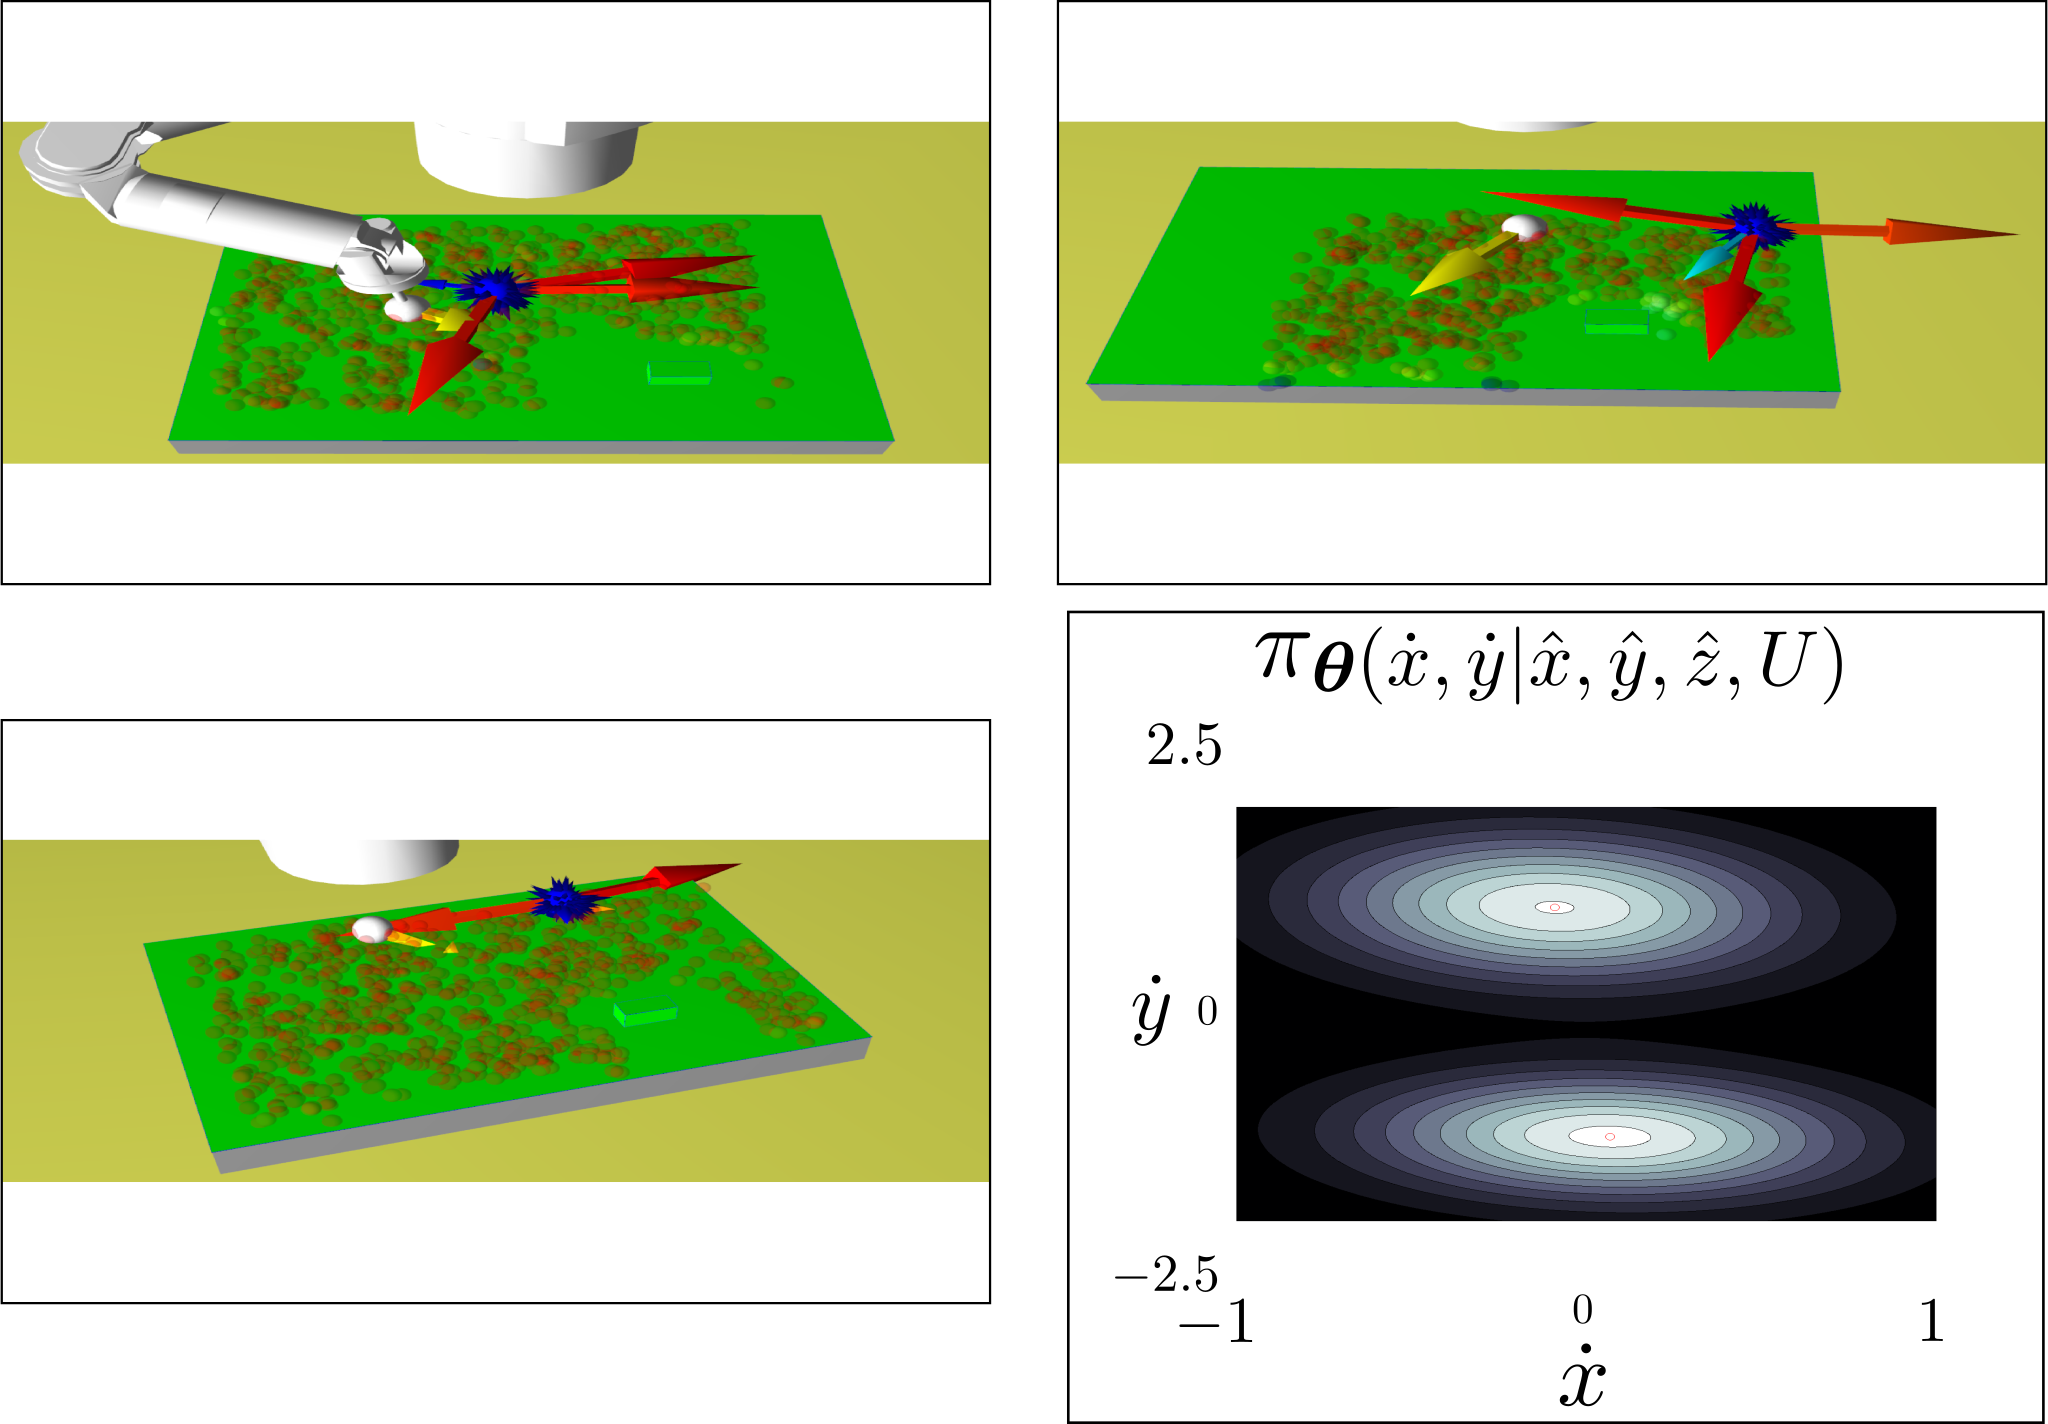
\includegraphics[width=0.95\textwidth]{./ch3-Search/Figures/Figure9_m}
    \caption{Illustration of three different types of modes present during the
    execution of the task where the robot is being controlled by the learned GMM model.
    The white ball represents the actual position of the robot's end-effector. The blue ball represents the
    believed position of the robot's end-effector and the robot is acting according to it. 
    The blue ball arrows represent modes. Colours encode the model's weights given by the priors $w^{[k]}$ after conditioning ( but not re-weighted as
    previously described). The spectrum ranges from red (high weight) to blue (low weight). \textit{Top left:} Three modes are present, but two agree with each other.   
    \textit{Top right:} Three modes are again present indicating appropriate ways to reduce the uncertainty. \textit{Lower left:} Two modes are in opposing directions. 
    No flipping behaviour between modes occurs since preference is given to the modes pointing in the same direction as the robot's current trajectory. \textit{Lower right:} GMM modes when conditioned on the state represented in the lower left figure.
    The two modes represent the possible directions (un-normalised).}
   \label{fig:modes}
\end{figure}

Figure \ref{fig:vectorfield} depicts the vector fields of both Coastal and GMM models where, as expected, the Coastal navigation 
trajectories tend to stay close to edges and corners until they are sufficiently close to the goal. This is achieved by weighting 
the information gain term $I(x_t)$ in the objective function sufficiently ($\lambda_2$). If $\lambda_2$=0 the Coastal policy is 
the same Greedy algorithm. 

It can be further seen that when the uncertainty tends towards it's maximum value ($U \rightarrow 1$) 
all behaviour tends to go towards the edges and corners. As the uncertainty reduces ($U \rightarrow 0$) the vector field 
tends directly towards the goal. However even at a low level of uncertainty, the behaviour at the edges and corners remains 
multi-modal and tends to favour remaining close to the edges and corners. 
This is an advantage of the GMM model. If the uncertainty has been sufficiently reduced and 
the true position of the end-effector or hand is not near an 
edge the policy dictates to go straight to the goal. This is not the case for the Coastal algorithm which ignores the 
uncertainty and strives to remain in the proximity of corners and edges until sufficiently close. 
This approach could potentially lead to unnecessary travel cost which could otherwise have been avoided.

\begin{figure}
  \centering
  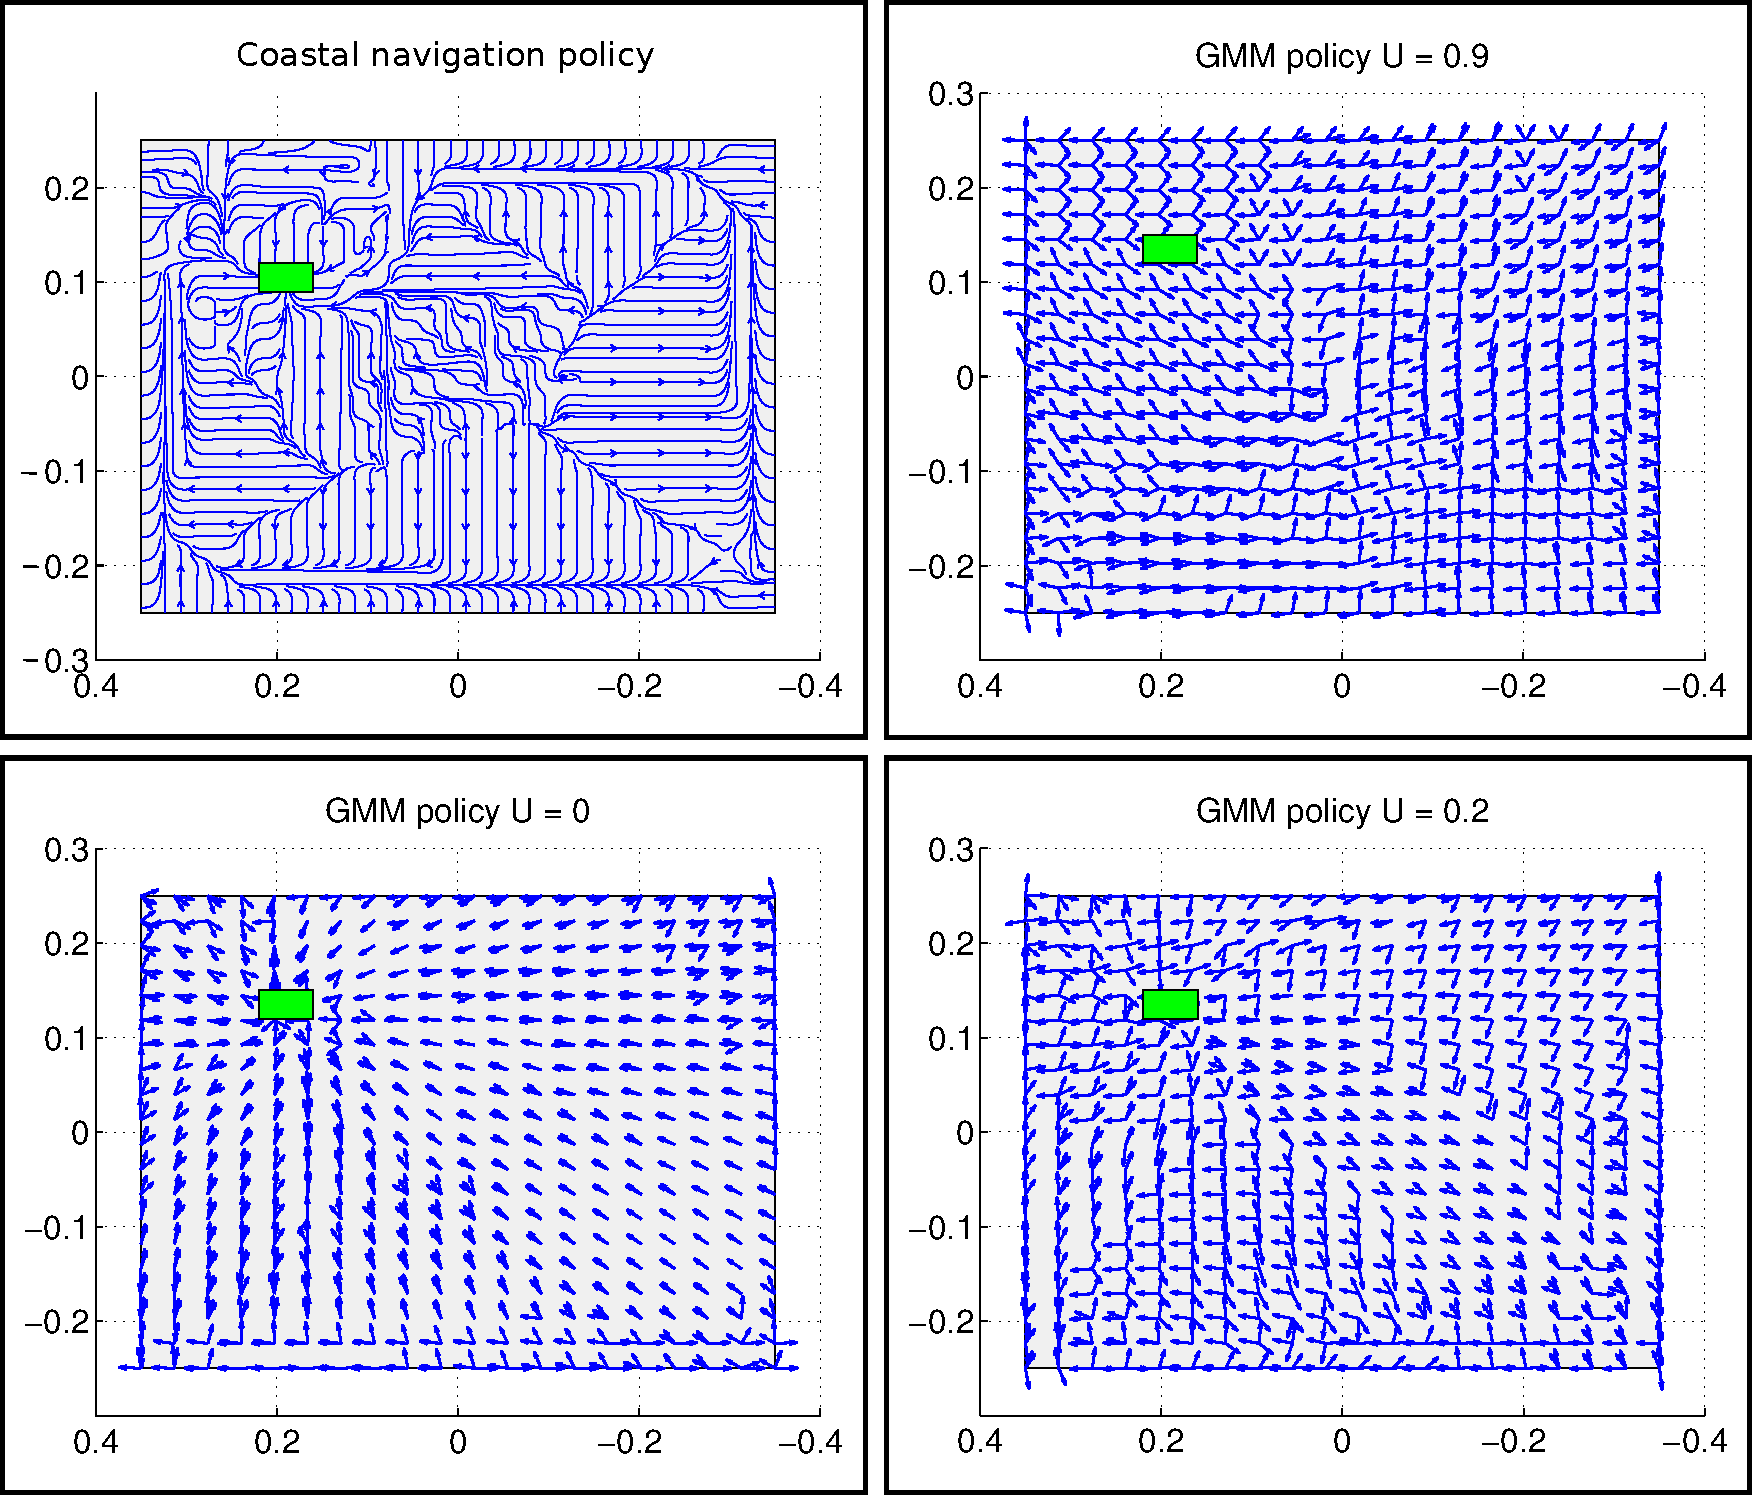
\includegraphics[width=0.95\textwidth]{./ch3-Search/Figures/Figure10}
  \caption{Illustration of the vector field for the Coastal and GMM policy. \textit{Top Left} Coastal policy, there is only one possible direction for every 
  state at any time, the values of $\lambda_2$ in the cost function were set experimentally. \textit{Others:} The GMM policy for three different levels of
  uncertainty. For each point multiple actions are possible which is reflected by the number of arrows (only the first three most likely actions). As 
  the uncertainty decreases the policy becomes less multi-modal, but remains around the edges and corners. Note that once certain
  of being close to an edge there is a possibility to go either straight to the goal or stay close to the edge and corners.}
  \label{fig:vectorfield}
\end{figure}

\FloatBarrier
\subsection{Distance efficiency \& Uncertainty}\label{sub:time_uncertainty}

We seek to distinguish the most efficient method in terms of two metrics, the distance (in meters) taken to reach the goal
and the level of uncertainty upon arriving at the goal. We report results on 5 different search 
experiments in which we compare the Greedy, GMM and Coastal Navigation algorithms. The Hybrid was not fully considered since it 
is a heuristic combination of the Greedy and GMM methods. 

In the first experiment, the true and believed locations of the end-effector 
were drawn uniformly from the original start distribution (Figure \ref{fig:experiment}, \textit{top right}) 
reflecting the default setting. The initializations (both real and believed end-effector locations) for the 
remaining 4 experiments were chosen in order to reflect particular situations which highlight the differences 
and drawbacks between each respective search method.
For the first experiment (Uniform search experiment), a 100 trials were carried out in which the end-effector position and belief were 
initialized uniformly. As for the other 4 search experiments, 40 separate runs were carried for each of the three algorithms.

\begin{figure}
   \centering
 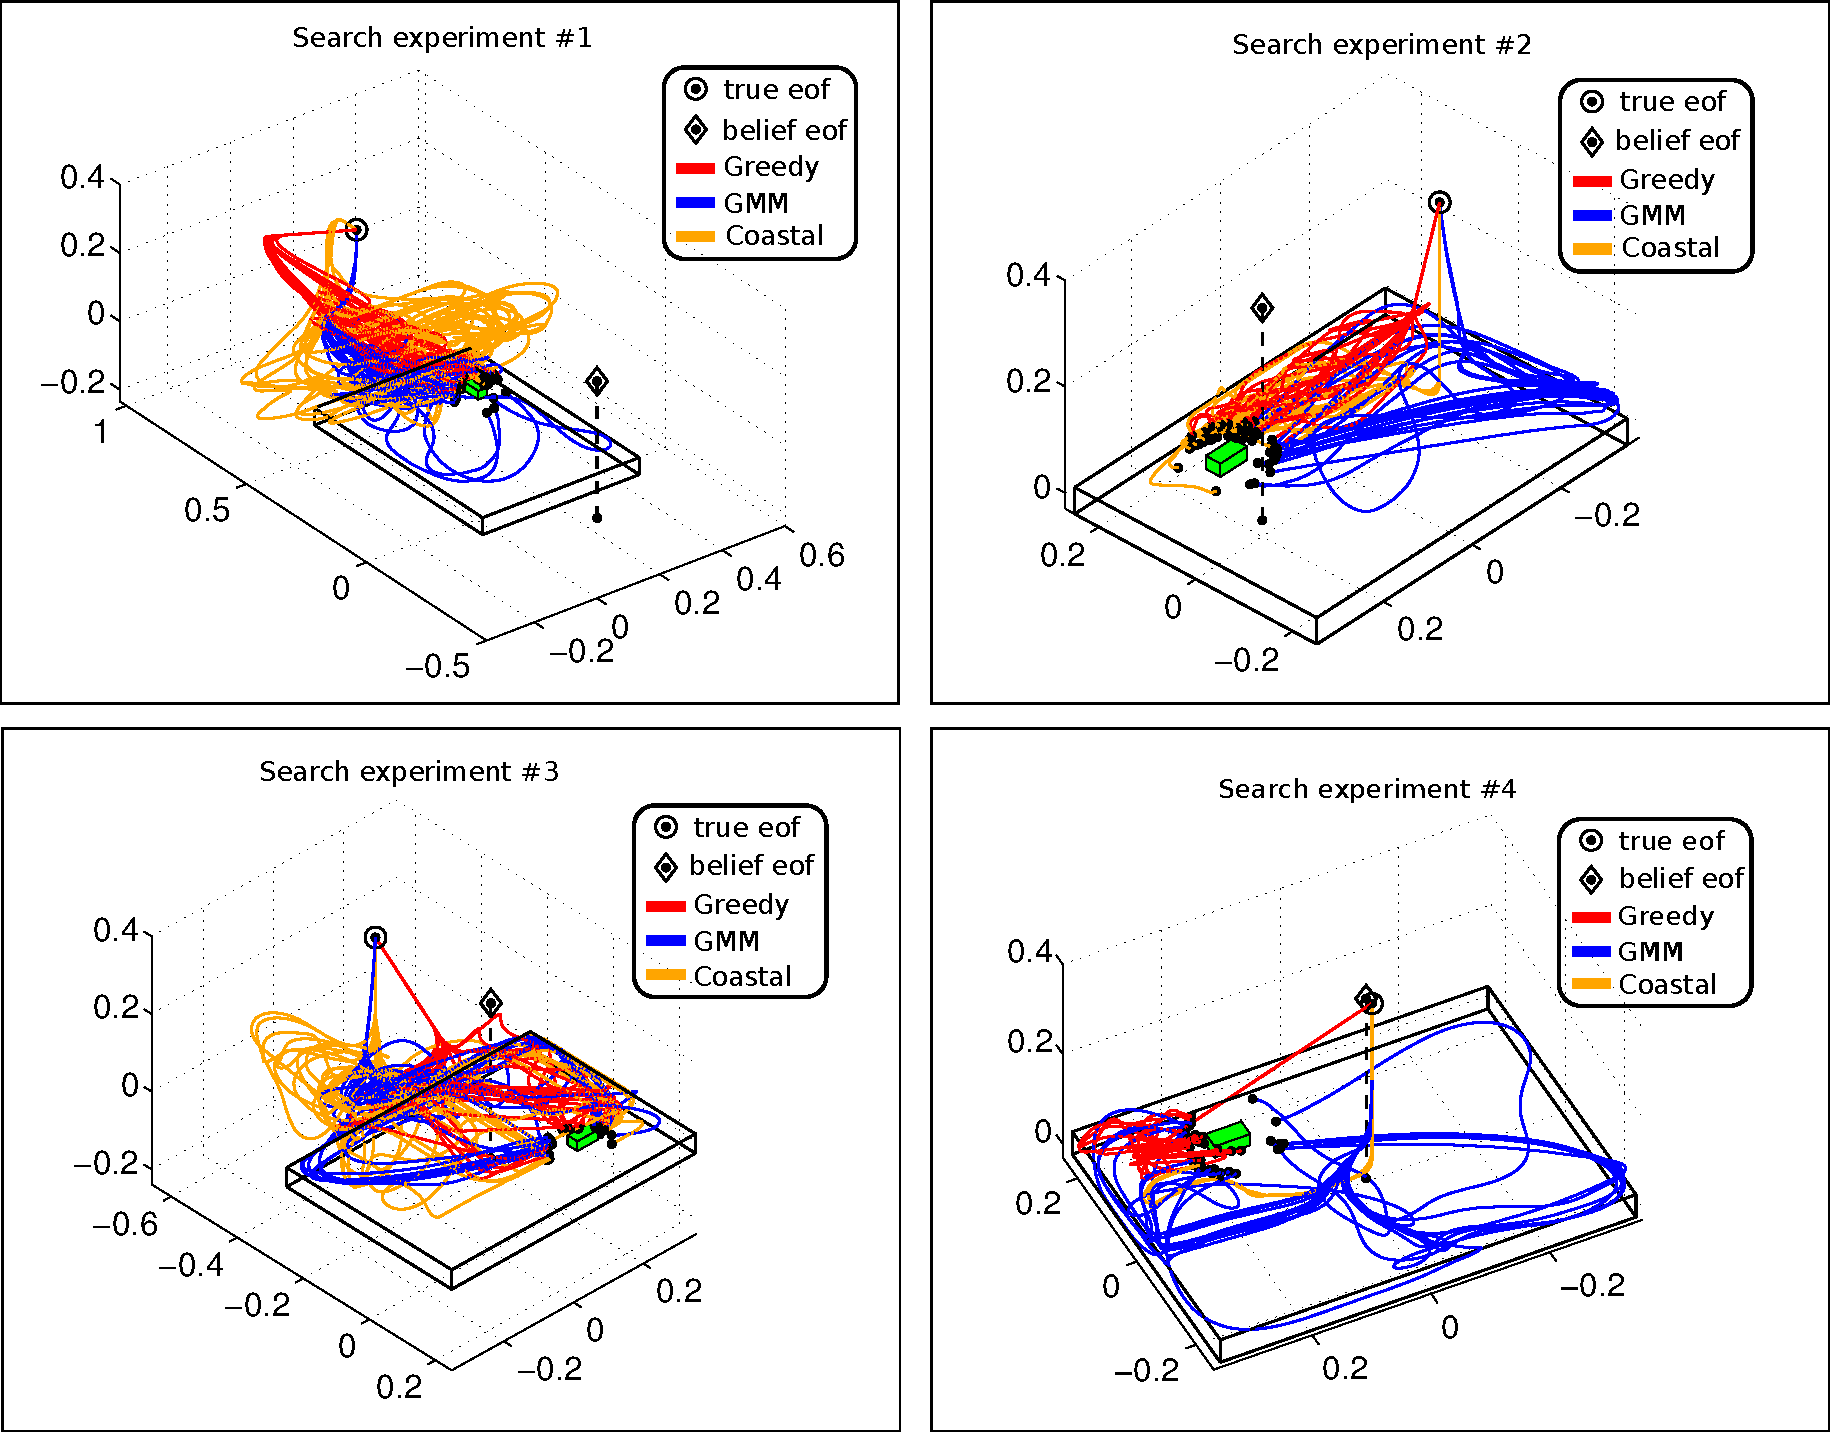
\includegraphics[width=\textwidth]{./ch3-Search/Figures/Figure11}
\caption{Four search initializations, from \textit{top left} to \textit{bottom right} we refer to them as \#1-4. The 
circle indicates the true starting point of the end-effector (eof), whilst the triangle is the initial believed location of the eof.
The initialisation in \#1 was chosen such that the true and believed eof locations were at opposite sides of the table. 
This setting was selected to highlight the draw back in methods which do not take into account uncertainty. 
The second initialisation \#2, reflects the situation where once again there is a large distance between true and believed location of 
the eof. However this time both are above the table. The starting points in \#3 are a variant on \#1 
with the difference being that the believed eof position is above the table whilst the true eof location is not. The last 
experiment \#4 was a setup which would be favourable to algorithms that are inclined to be greedy. Both true and believed 
eof locations are close to one another.}
\label{fig:four-initialisations}
\end{figure}

Table \ref{tab:mean-var-distance} reports the mean and variance of the distance taken (in meters) to reach the goal for each search 
method for all 5 experiments.
We report on an Analysis of Variance (ANOVA) to test that all experiments were 
significantly different from one another as were the searches. We test the null hypothesis,  $H_o$,  that there is 
no statistical difference between the 5 search experiments. 
Before performing the ANOVA, we verified that our dependent variable, distance [m] taken to reach the goal, follows a normal 
distribution for all methods and all experiments (a total of $5 \times 3 = 15$ tests), an assumption which is required by 
an ANOVA analysis. A Kolmogorov-Smirnov test was performed on each experiment and associated search method. A total 
of 11/15 searches rejected the null hypothesis with a significance level of less than 5\% (p-value $<$ 0.05). 

\begin{table}
 \centering
  \begin{tabular}{|c|c|c|c|c|}     
  \hline
      Experiment       &  \textbf{Greedy}      	  	&  \textbf{GMM}      		&  \textbf{Coastal}     \\\hline
       Uniform         &   1.54 (0.46) 	  		& 0.99 (0.14) \cellcolor{Gray} 	& 1.13 (0.57)    \\
	\#1            &   3.02 (0.36)    		& 1.82 (0.23) \cellcolor{Gray} 	& 3.44 (1.50)    \\
	\#2            &   0.80 (0.01) \cellcolor{Gray} & 1.41 (0.14) 			& 0.94 (0.01)    \\
	\#3            &   1.14 (0.08) \cellcolor{Gray} & 1.80 (0.17) 			& 2.14 (0.81)    \\
	\#4            &   0.75 (0.04)  		& 1.34 (0.07) 			& 0.68 (0.01) \cellcolor{Gray} \\ \hline
 \end{tabular}
  \caption{Mean distance and (variance) taken to reach the goal for 3 methods in 5 experiments. The grey shaded entries correspond to the results of the search algorithm 
  which obtained the fastest time to reach the goal in each type of experiment/search.}
  \label{tab:mean-var-distance}
\end{table}

In Table \ref{tab:anova-1} we report the p-values and F-statistics for an ANOVA on the 5 different experiments where our 
null hypothesis is that all experiments produce statistically the same type of search. For all experiment types the p-value 
is extremely small, below a significance value of 1\% (p-value $<$ 0.01) which indicates that we can safely reject the 
null hypothesis and accept that all experiments produced very different searches, which is important for a 
comparative study.

\begin{table}
 \centering
  \begin{tabular}{|c|c|c|c|c|c|}
  \hline
   search method &  Uniform       &   \#1	   & 	\#2	     & 	    \#3	       &   \#4 \\ \hline
   p-value (F)   &  2e-06 (14) & 5e-07 (19) &  7e-11 (36) &  4-06 (15) &  4e-16 (67) \\ \hline
 \end{tabular}
 \caption{ANOVA tests the null hypothesis that all search experiments produced the same type of search with respect to the distance taken to reach the goal. 
 All the p-values are extremely small which indicate that the null hypothesis can safely be rejected.}
 \label{tab:anova-1}
\end{table}

As the first ANOVA only indicated that the experiments produced different searches,
we also performed a second ANOVA test between the paired search methods to confirm that the methods themselves are statistically different.
Table \ref{fig:anova-2} illustrates the difference between the individual search methods for each experiment. 
It was found that most search algorithms produced significantly different searches (p-value $<$ 0.01) with
the exception of the GMM and Coastal algorithm for the Uniform and \#3 experiment (p-value $<$ 0.1). 
However the GMM and Coastal trajectories for the \#3 experiment appear to be quite different when the trajectories 
are off the table's surface, see Figure \ref{fig:four-initialisations} \textit{(Bottom left)}, but share similar 
characteristics such as edge following behaviour.

\begin{table}
 \centering
 \begin{tabular}{|c|c|c|c|}
 \hline
   p-value (F)   &  Greedy vs GMM      &     Greedy vs Coastal        &  GMM vs Coastal     \\\hline
  Uniform & 3.59e-08 (30)  &   3.32e-04 (13) 		     &  1.90e-01 (2)  \cellcolor{Gray}\\
\#1  	  & 5.80e-08 (46) &  1.88e-01 (2) \cellcolor{Gray} &  4.58e-06 (28)\\
\#2	  & 3.60e-08 (47) &  4.68e-04 (14)		    &  4.54e-06 (28) \\
\#3	  & 3.57e-07 (37) &  2.07e-05 (23)		    &  1.25e-01 (2) \cellcolor{Gray} \\
\#4	  & 6.70e-10 (64) &  1.58e-01 (2) \cellcolor{Gray} &  6.34e-13 (107) \\ \hline
\end{tabular}
\caption{ANOVA between paired search methods. The first column gives an indication of the probability that both the Greedy 
and GMM searches are statistically the same (the null hypothesis). This was rejected with a tolerance of below \%1. 
In the second column, Greedy vs Coastal searches \#1 and \#4 are statistically closer 
than the rest with a p-value threshold of 10\% required to be able to reject the null hypothesis. 
In the third column the uniform and \#3 are not statistically different and would require a higher threshold on the p-value to be so.}
\label{fig:anova-2}
\end{table}

From our ANOVA analysis we conclude that the behaviour exhibited by the three search strategies is 
significantly different. This is certainly the case for the Greedy and GMM methods, even though in 
certain situations the Greedy and Coastal policies display similar behaviour such as in experiment \#1.
The reason for this is that both the Greedy and Coastal policies start in a situation where there are no salient features available
and their polices take the true end-effector location to an even more feature deprived 
region. In this situation the GMM policy is the clear winner with respect to the distance taken to reach
the goal. 

In experiment \#2, both Greedy and Coastal policies perform equally well, and usually perform faster than the GMM model if the true 
and believed locations of the end-effector remain on the surface of the table. Otherwise if this is not the 
case, they will both reduce the uncertainty in a very inefficient way as the modes will often change during the search. 
This leads to the believed position (most likely state, $\hat{x}_t$) varying greatly, resulting in an increased time before the uncertainty 
has been narrowed down sufficiently for a contact to occur with the table (or simply by chance).


\begin{figure}
   \centering
  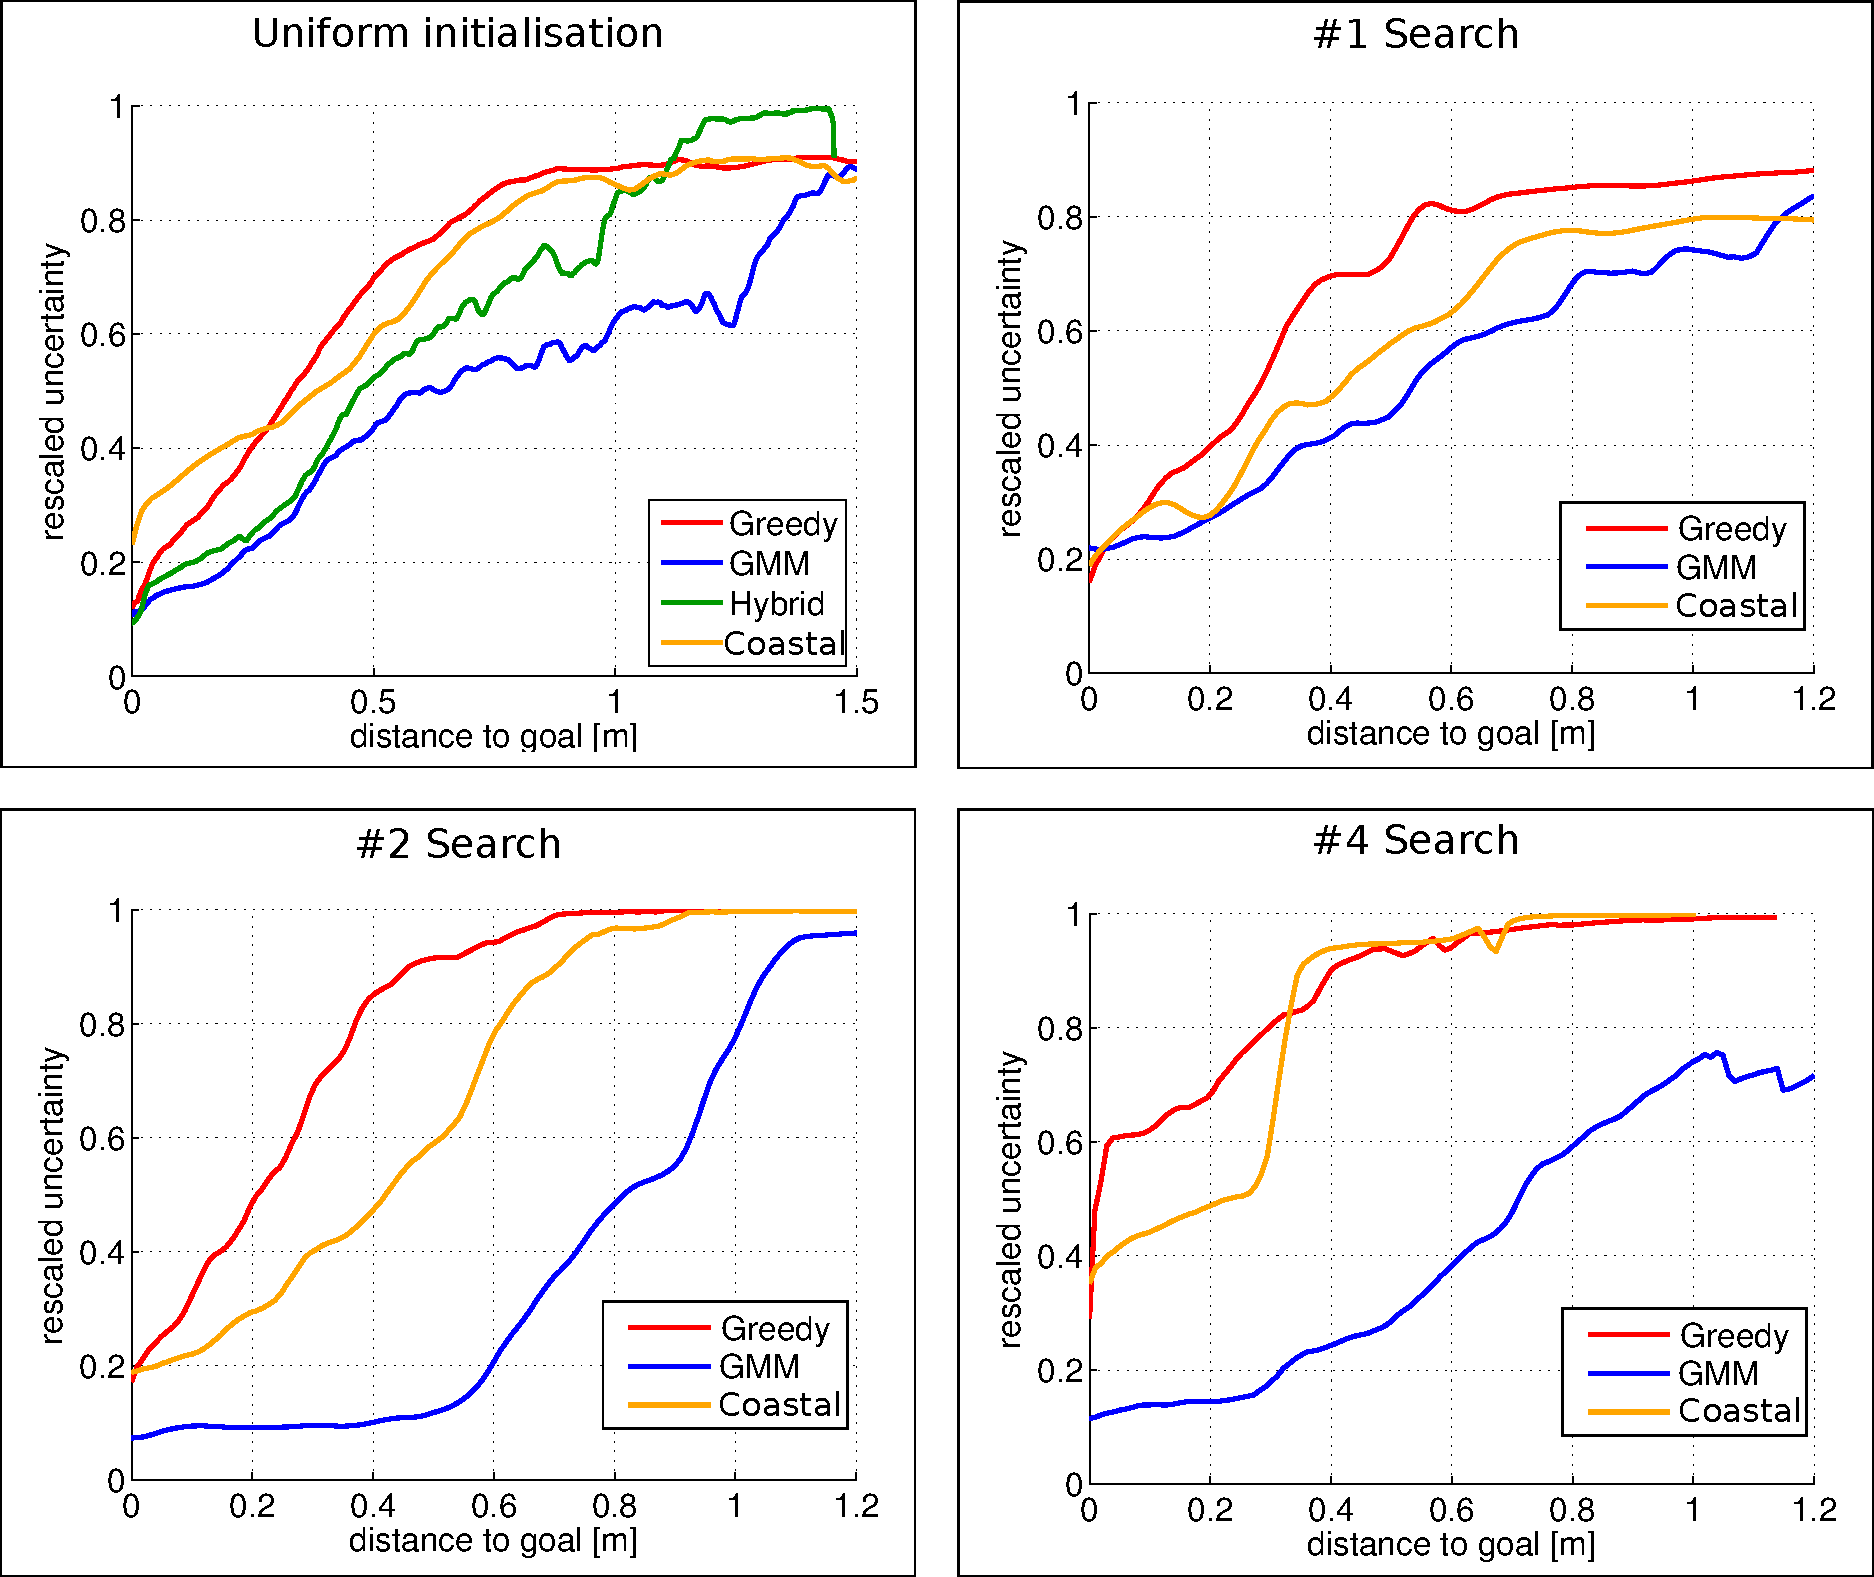
\includegraphics[width=0.95\textwidth]{./ch3-Search/Figures/Figure12}
\caption{Reduction of the uncertainty for the Uniform, \#1, \#2 and \#4 experiment, the expected value is reported
\textit{Top left}: Uniform initialisation, expected uncertainty for the Greedy (red), GMM (blue), Hybrid (green) \& Coastal (orange) search
 strategies.
\textit{Top right:} Experiment \#1. \textit{Bottom left:} Experiment \#2. \textit{Bottom right:} Experiment \#4.}
\label{fig:uncertainty}
\end{figure}


Figure \ref{fig:uncertainty} shows the normalised uncertainty with respect to the distance remaining to the goal for all experiments, 
(\#3 is excluded being similar to the \#2). 

The results show which methods actively minimise the uncertainty and which methods find the goal whilst being more dependent on chance. 
For all the reported experiments the GMM (learned from human searches) reaches a lower expected uncertainty than all other search algorithms. 
For the Uniform and \#1 search experiment, all methods reach the same final uncertainty level. However, for the \#2 and \#4 experiments, 
the GMM reaches the goal with significantly lower uncertainty. It is inferred that the GMM model actively minimises the uncertainty 
which is also reflected in the distance it takes to reach the goal in comparison with the other methods.

While  the Greedy (\#2) and Coastal (\#4) are faster than the GMM method, Table \ref{tab:mean-var-distance}, both have a far higher level 
of uncertainty at the arrival which leads to the assumption that chance has a non-negligible effect on their success. 



%%%%%%%%%%%%%%%%%%%%%%%%%%%%%%%%%%%%%%%%%%%%%%%%%%%%%%%%%%%%%%%%%%%%%%%%%%%%%%%%%%%%%%%%%%%%%%%%%%%%%%%%%%%%%%%%%%%%%%%%%%%%%%%%%%%%%%%%%
%																	%
%				Conclusion 		 										%
%																	%
%%%%%%%%%%%%%%%%%%%%%%%%%%%%%%%%%%%%%%%%%%%%%%%%%%%%%%%%%%%%%%%%%%%%%%%%%%%%%%%%%%%%%%%%%%%%%%%%%%%%%%%%%%%%%%%%%%%%%%%%%%%%%%%%%%%%%%%%%

\FloatBarrier
\section{Conclusions}

In this work we have shown a novel approach in teaching a robot to act in a partially observable environment. 
Through having human volunteers demonstrate the task of finding an object on a table, we recorded both the 
inferred believed position of their hand and associated action (normalised velocity). A generative model
mapping the believed end-effector position to actions was learned, encapsulating this relationship. 
As speculated and observed, multiple strategies are present given a specific belief. This can be interpreted as the fact that 
humans act differently given the same situation. 

The behaviour recorded from the human demonstrations, encoded as set of expected sensations, showed
the presence of trajectories which both remained near to the edge and corner features but also 
trajectories which remained at a distance. Risk-prone and risk-averse behaviour was further 
confirmed by the overlap of the risk factor of Human and GMM generated trajectories with that of the Greedy
risk factor. According to the feature-based factor, more than 70\% of the human search trajectories were considered
to be risk-averse whilst 93\% according to the Risk factor. Similarly the GMM search trajectories showed to be
89-88\% risk-averse.

In terms of the comparative study, the GMM controller is more adapted to dealing with situations of high uncertainty and 
accounts for it better than Greedy or Coastal planning approaches. This is evident in the experiment
where the believed position and true position of the end-effector were significantly far apart and distant from salient areas. 
Future questions of scientific value to be addressed are to which extent do humans follow the reasoning 
of a Markov Decision Process in a partially observable situation where the state space is continuous 
(the problem has been partially addressed in \cite{Bake_Saxe_Tene_2011} for discrete states and actions). 

A drawback of the PbD-POMDP approach is that the quality of the learned policy is dependent on the abilities 
of the human teacher. If the teacher is consistent and goal directed (on average) then the transferred policy will be adequate, if however
the human is suboptimal at performing the task, then the resulting policy will be poor. An autonomous way of
evaluating the quality of the demonstrations whilst learning a policy is necessary. In the next chapter, ``Chapter 4'', we 
demonstrate that by introducing a cost function and using a Reinforcement Learning approach we can account
for poor demonstrations and increase the quality of the policy.


%A further aspect of interestis to study the situation where multiple beliefs are present and investigate how humans 
%perform simultaneous localization and mapping as opposed to active localization which was the area of interest of 
%this research. 


% Basically talk about the drawback and introduce the next chapter.












